


\subsection{Fore-aft tower model fitting} \label{sec:app_mod_foreaft_fitting}
As described in \hyperref[sec:comp_foreaft_mod]{\textbf{fore-aft tower model}} \cref{sec:comp_foreaft_mod} the component which models the fore-aft movement consists of a simple second order mass-spring-damper system. This simplified model consists of only three parameters: A mass $ m $, a spring constant $ k $ and a damper constant $ b $. Setting these parameters such that the model fits the behaviour of the real system well is not intuitive. When the model equations were written on the standard second order TF form it became apparent that the parameters could be derived from the mass, the natural frequency $ \omega_n $ and the dampening factor $ \zeta $. While these parameters are much more intuitive to place some tuning still has to be done. This section is dedicated to explaining the tuning procedure and showcasing the final results of the tuning process. The starting point for the parameter estimation was as follows:

\smallskip
\noindent Setting the \textbf{natural frequency} around the eigenfrequency of the turbine is a good place to start. Thus $ \omega_{ninit} = 0.035 \cdot 2 \pi $.

\smallskip
\noindent A first guess for the \textbf{effective mass} $ m $ is the combined mass of: The tower, nacelle, hub and rotor blades. This is simply a rough estimate which is not expected to yield satisfactory results mainly because the mass M does not represent the actual mass of the system but rather the inertia of the pitching of the whole structure in the water. Thus $ m_{init} = m_{tower} + m_{hub} + m_{nacelle} + 3 \cdot m_{blade} = 77743 + 82262 + 293382 + 3*36251 $

\smallskip
\noindent Many factors affect the \textbf{dampening} of the fore-aft movement. As described in \cref{sec:intro_theFOWT} ballast, buoyancy and mooring line forces all contribute to the stability and dampening of the fore-aft tower movement. Furthermore as also described in \cref{sec:theory_fowt_challenges} the rotor blades act as a sail which dampens the movement in the surge direction. A low dampening factor $ \zeta $ is assumed as a start since the dampening from the blades is modelled in the \hyperref[sec:comp_aero_thrust]{\textbf{aerodynamic thrust model}} \cref{sec:comp_aero_thrust}. Thus the only contributors to dampening of the system are from the other mentioned forces. Thus $ \zeta_{init} = 0.2 $

\medskip
In order to be able to fit the model to the real system it is of course necessary to have some data to fit it against.

\subsubsection*{System identification}
A Vestas tool is utilized to get frequency response plots of the real system from specific actuator inputs to any sensor in the simulation environment. The tool functionality can be split into two main parts. 

\textbf{Firstly} setup files are generated which alter the VTS simulation environment such that a sinusoid of chosen frequency and amplitude is induced on a chosen reference. A full simulation is run for every frequency. A preliminary test was made where the system behaviour was analysed when frequencies were induced, in the appendix in \cref{app:tj_00}. In this test only a few frequencies were induced on the rotor speed reference and the effect on the rotor speed and fore-aft motion was commented.

The \textbf{second part} is the processing of the simulation output data to plot frequency responses from the actuator to an output sensor. 

Furthermore for the parameter tuning the input actuators were chosen to be the generator speed reference and the pitch angle reference and the observed outputs were the measured generator speed and the tower top velocity. 60 different frequencies were spaced logaritmacally between 0.01 Hz and 0.3 Hz. The amplitude of the sinusoid was set to 5\% of the mean generator speed reference and and 1 degree for the rotor pitch. 

\subsubsection*{Fitting results}
In this subsection the results of the fitting process are presented. Firstly the model is fitted for the transfer function from rotor speed reference to rotor speed and from rotor speed reference to surge direction velocity. Secondly the model is fitted for the transfer function from the pitch reference to the surge direction velocity.

\smallskip
After a trail and error fitting process the parameters that were found to yield the most satisfactory fit were the following:
\begin{equation*}
	\begin{split}
		\omega_n &= 1.15 \, \omega_ninit \\
		m 		 &= 2.5 \, m_{init} \\
		\zeta 	 &= 0.13
	\end{split}
\end{equation*}


\begin{figure*}[ht]
	\centering
	
	\subfloat[VTS frequency response]{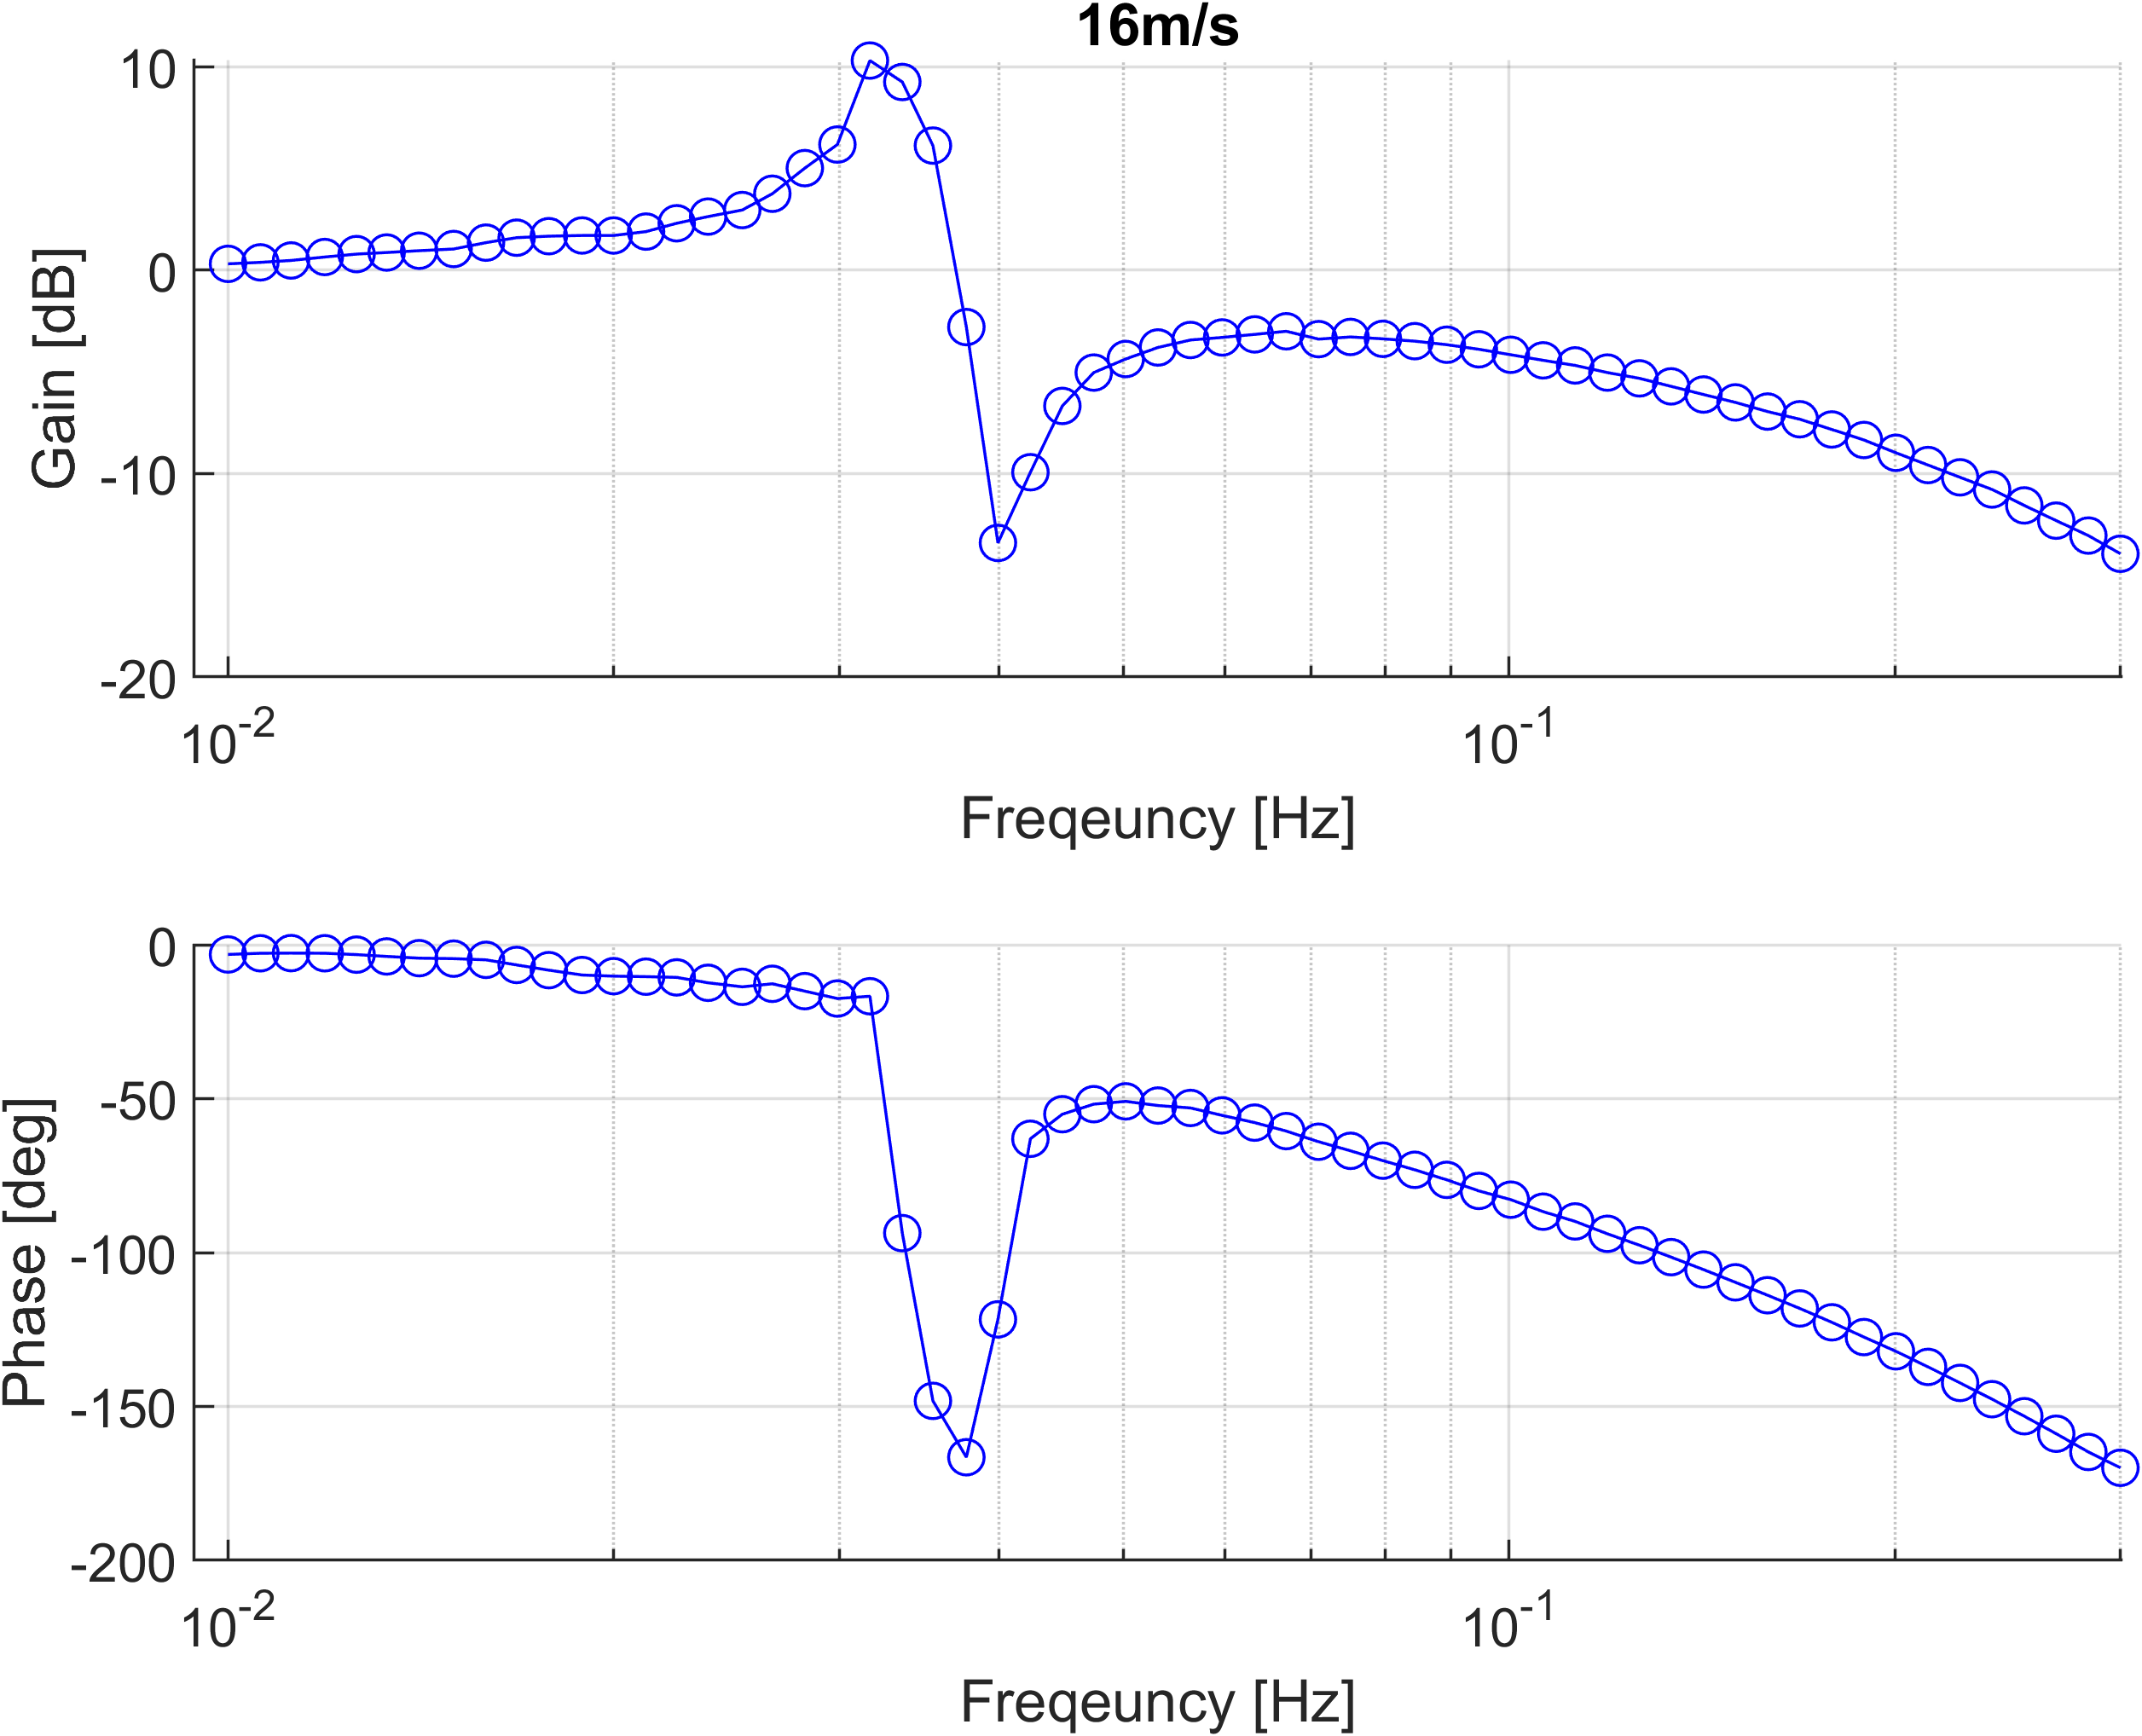
\includegraphics[width=.49\textwidth]{Graphics/TestResults/foreaftFitting/sysid_wRef-w_16ms.png}
		\label{fig:app_sysid_wref-w_16}}
	\hfil
	\subfloat[Linear model response]{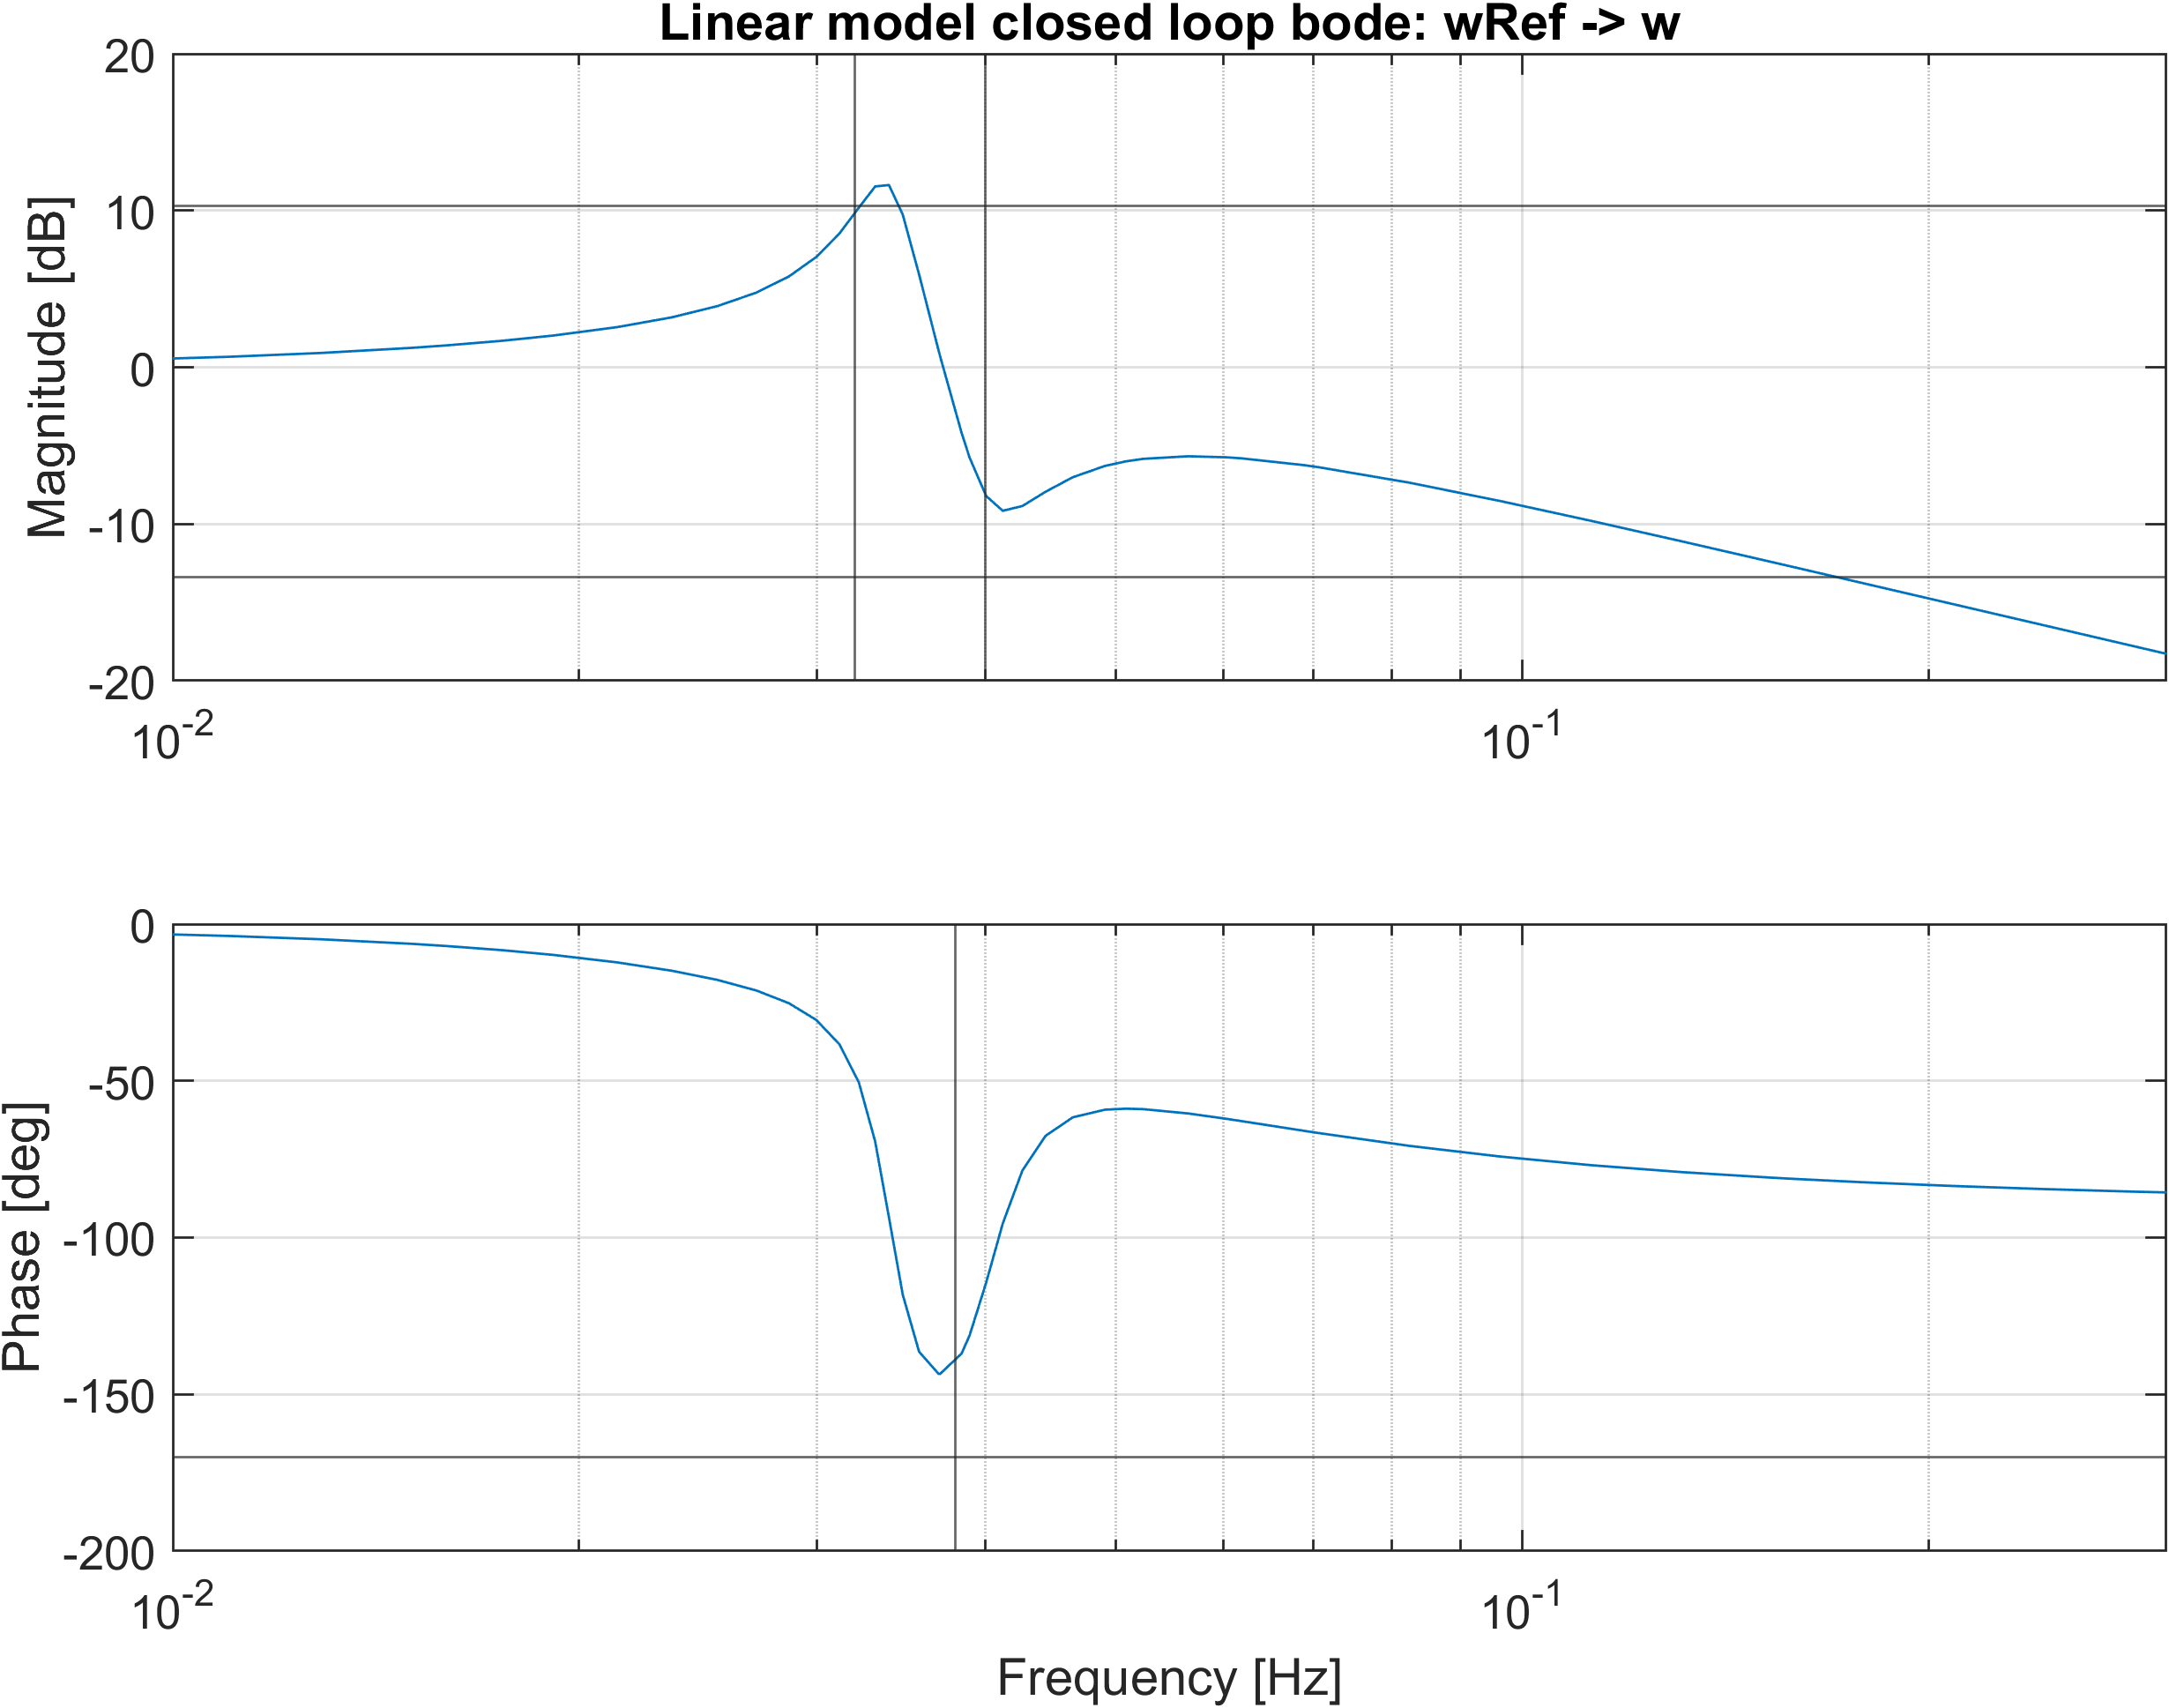
\includegraphics[width=.49\textwidth]{Graphics/TestResults/foreaftFitting/wtLin_wRef-w_16ms.png}
		\label{fig:app_wtlin_wref-w_16}}
	
	\caption{generator speed reference to generator speed fitting with operating point at 16 m/s; \textbf{(a)} VTS bode plot; \textbf{(b)} Linear model bode plot. Black lines are placed in the magnitude plot to indicate the peaks and valleys around the eigenfrequency and in the phase plot at the valley from (a).}
	\label{fig:app_wref-w_16}
\end{figure*}



\begin{figure*}[ht]
	\centering
	
	\subfloat[VTS frequency response]
	{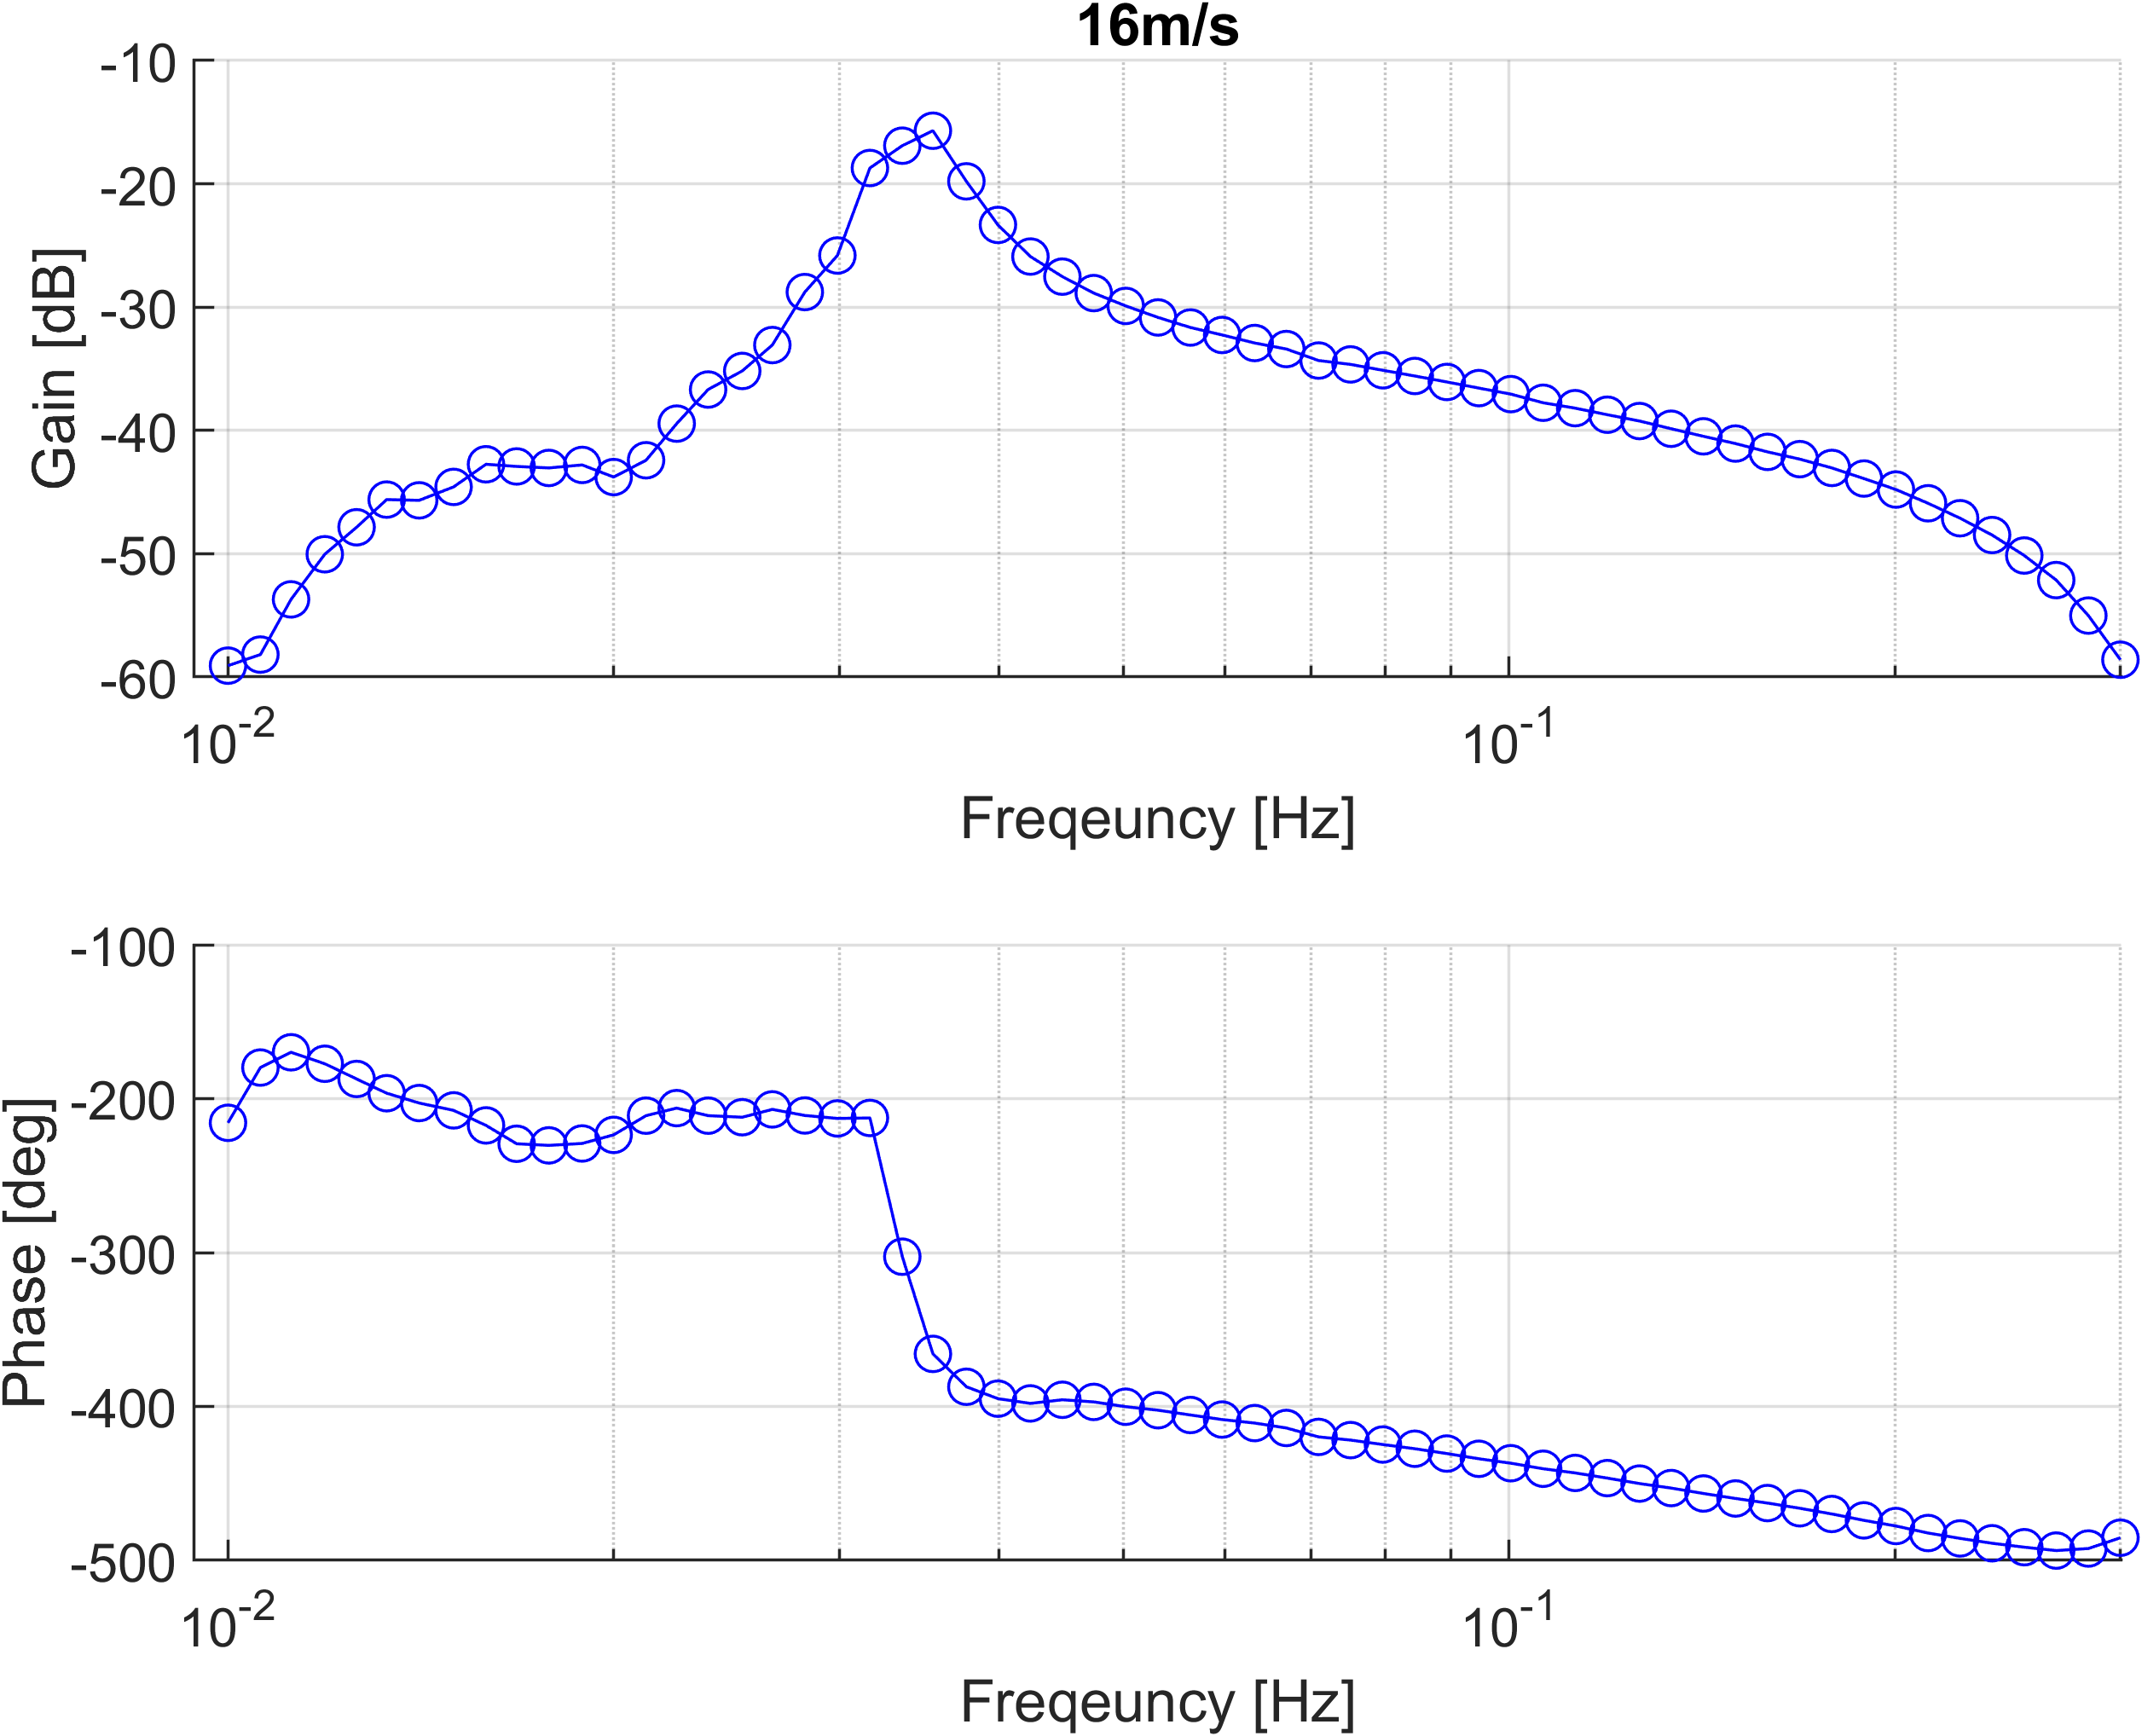
\includegraphics[width=.49\textwidth]{Graphics/TestResults/foreaftFitting/sysid_wRef-vy_16ms.png}%
			\label{fig:app_sysid_wref-vy_16}}
	\hfil
	\subfloat[Linear model response]
	{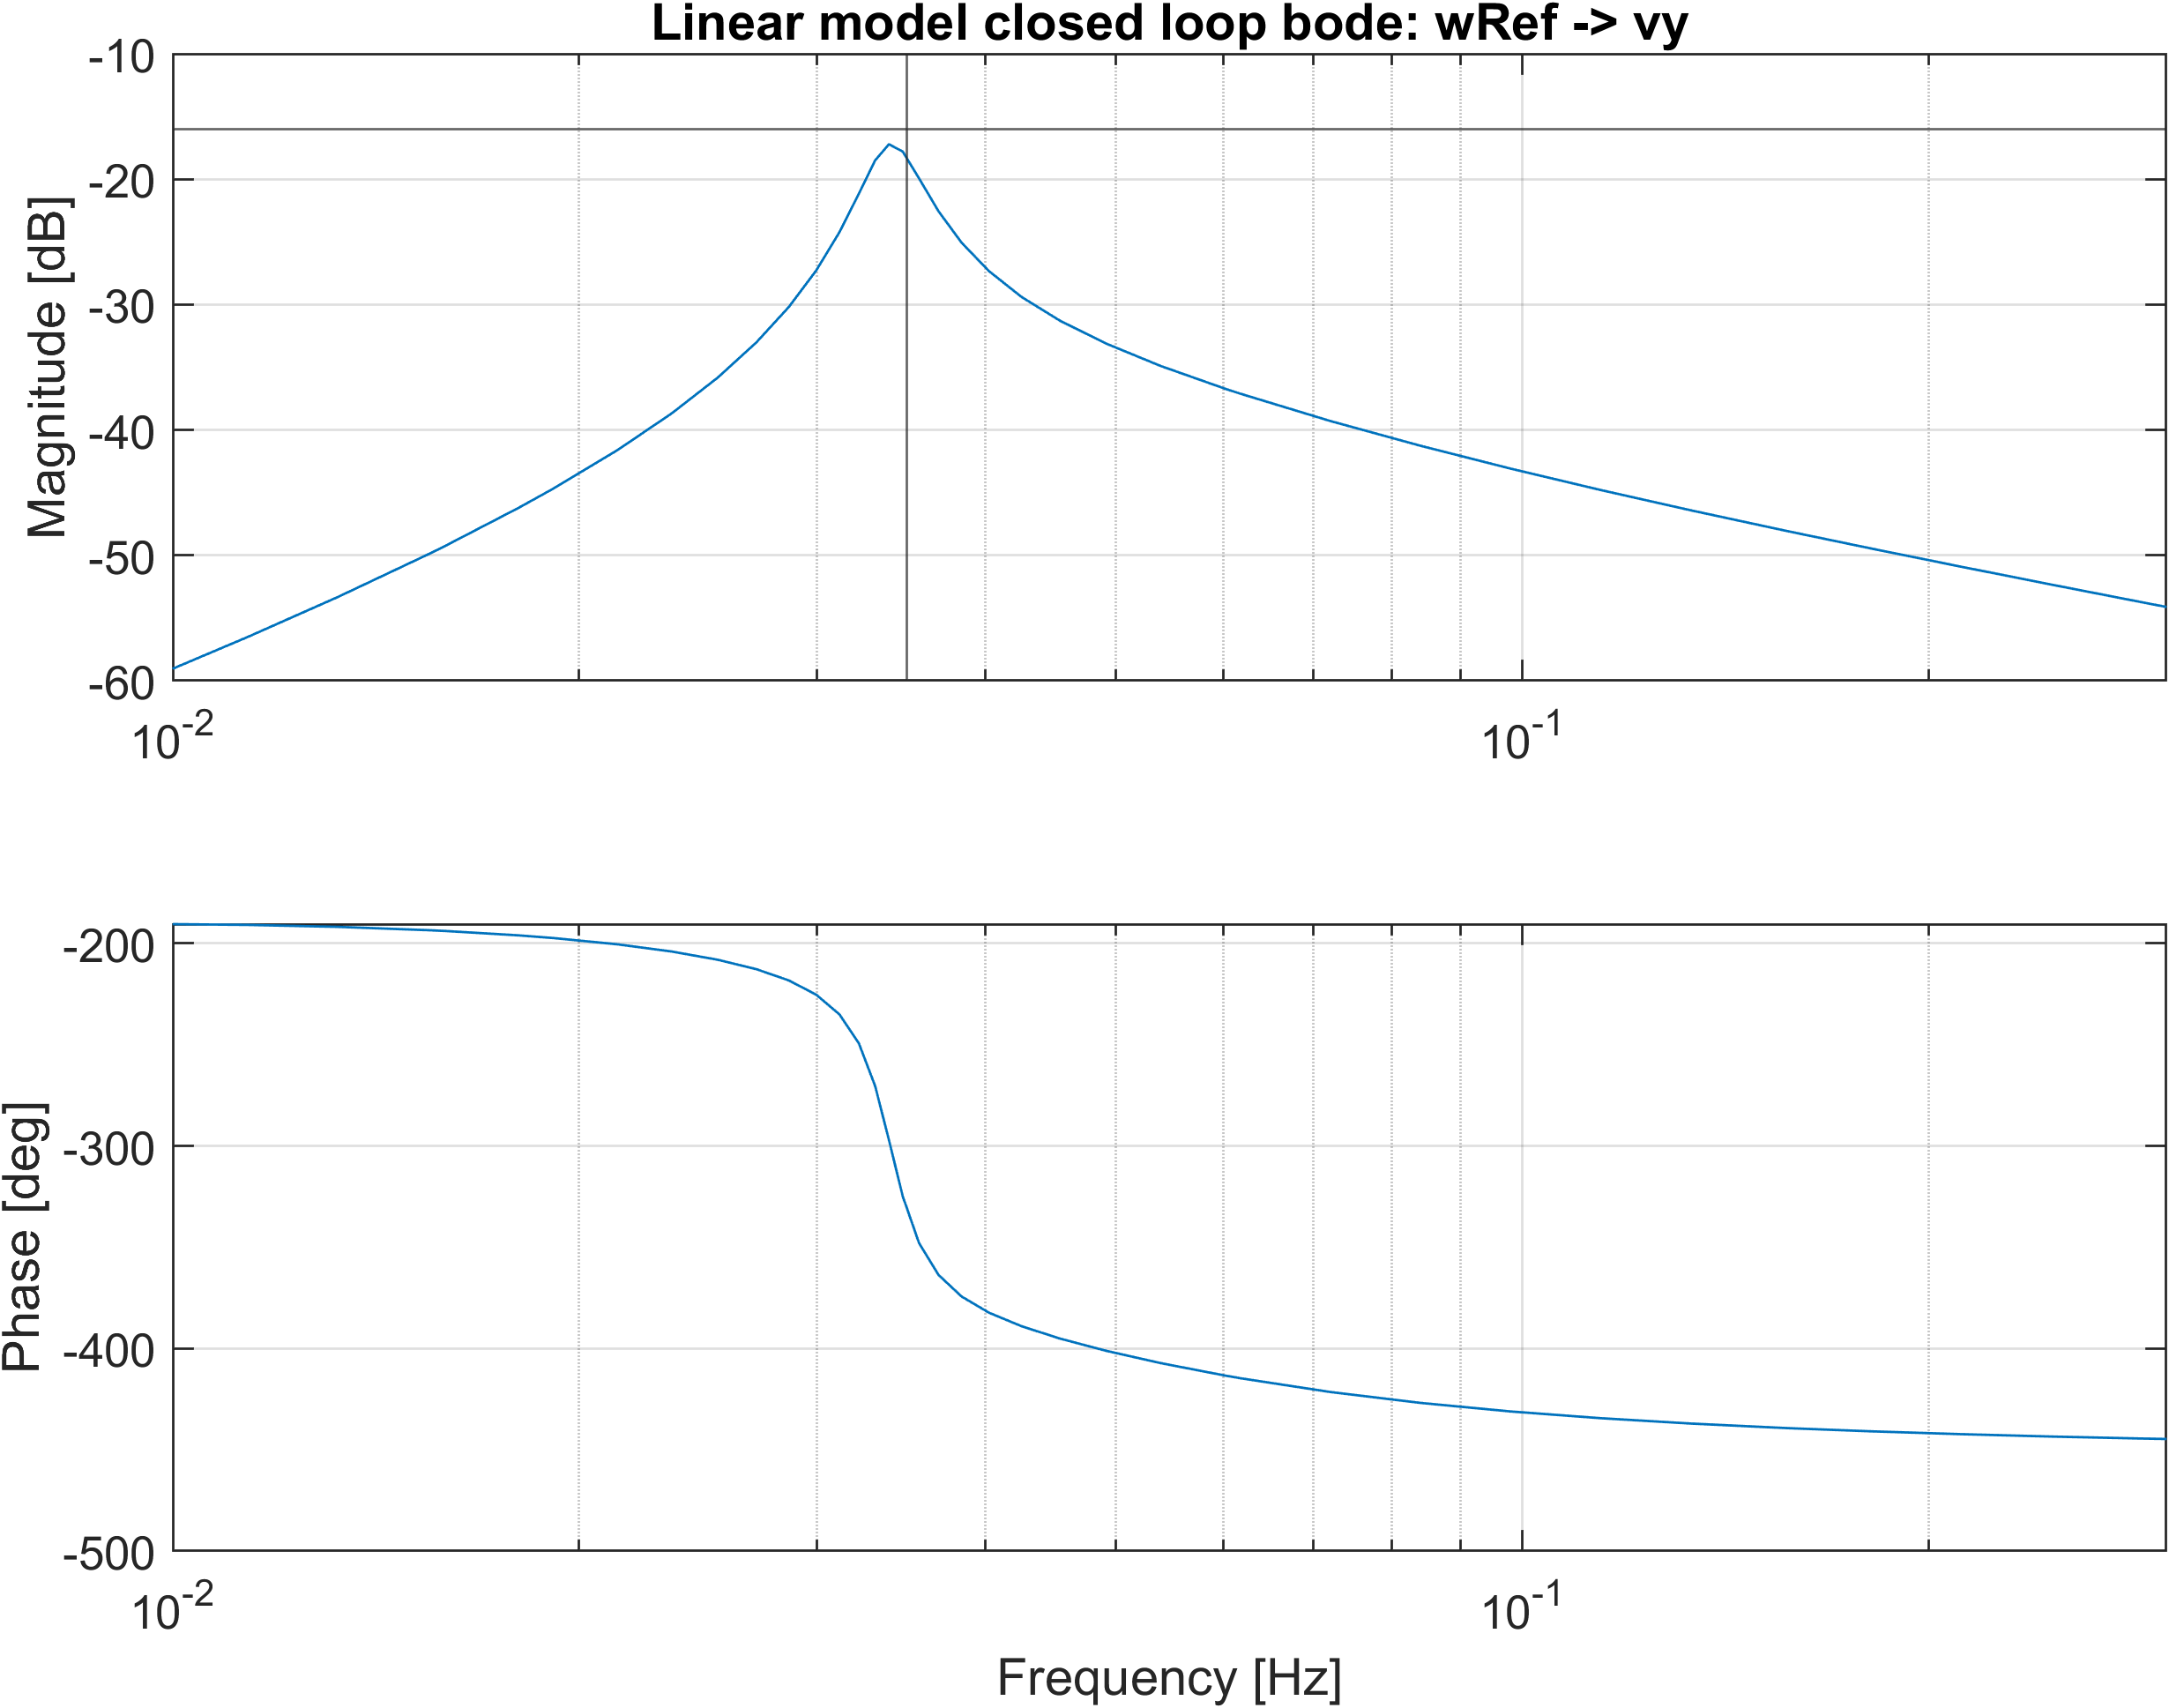
\includegraphics[width=.50\textwidth]{Graphics/TestResults/foreaftFitting/wtLin_wRef-vy_16ms.png}%
			\label{fig:app_wtlin_wref-vy_16}}
	
	\caption{generator speed reference to fore-aft surge velocity fitting with operating point at 16 m/s; \textbf{(a)} VTS bode plot; \textbf{(b)} Linear model bode plot. Black lines are placed in the magnitude plot to indicate position of magnitude peak from (a).}
	\label{fig:app_wref-vy_16}
\end{figure*}


\begin{figure*}[ht]
	\centering
	
	\subfloat[VTS frequency response]{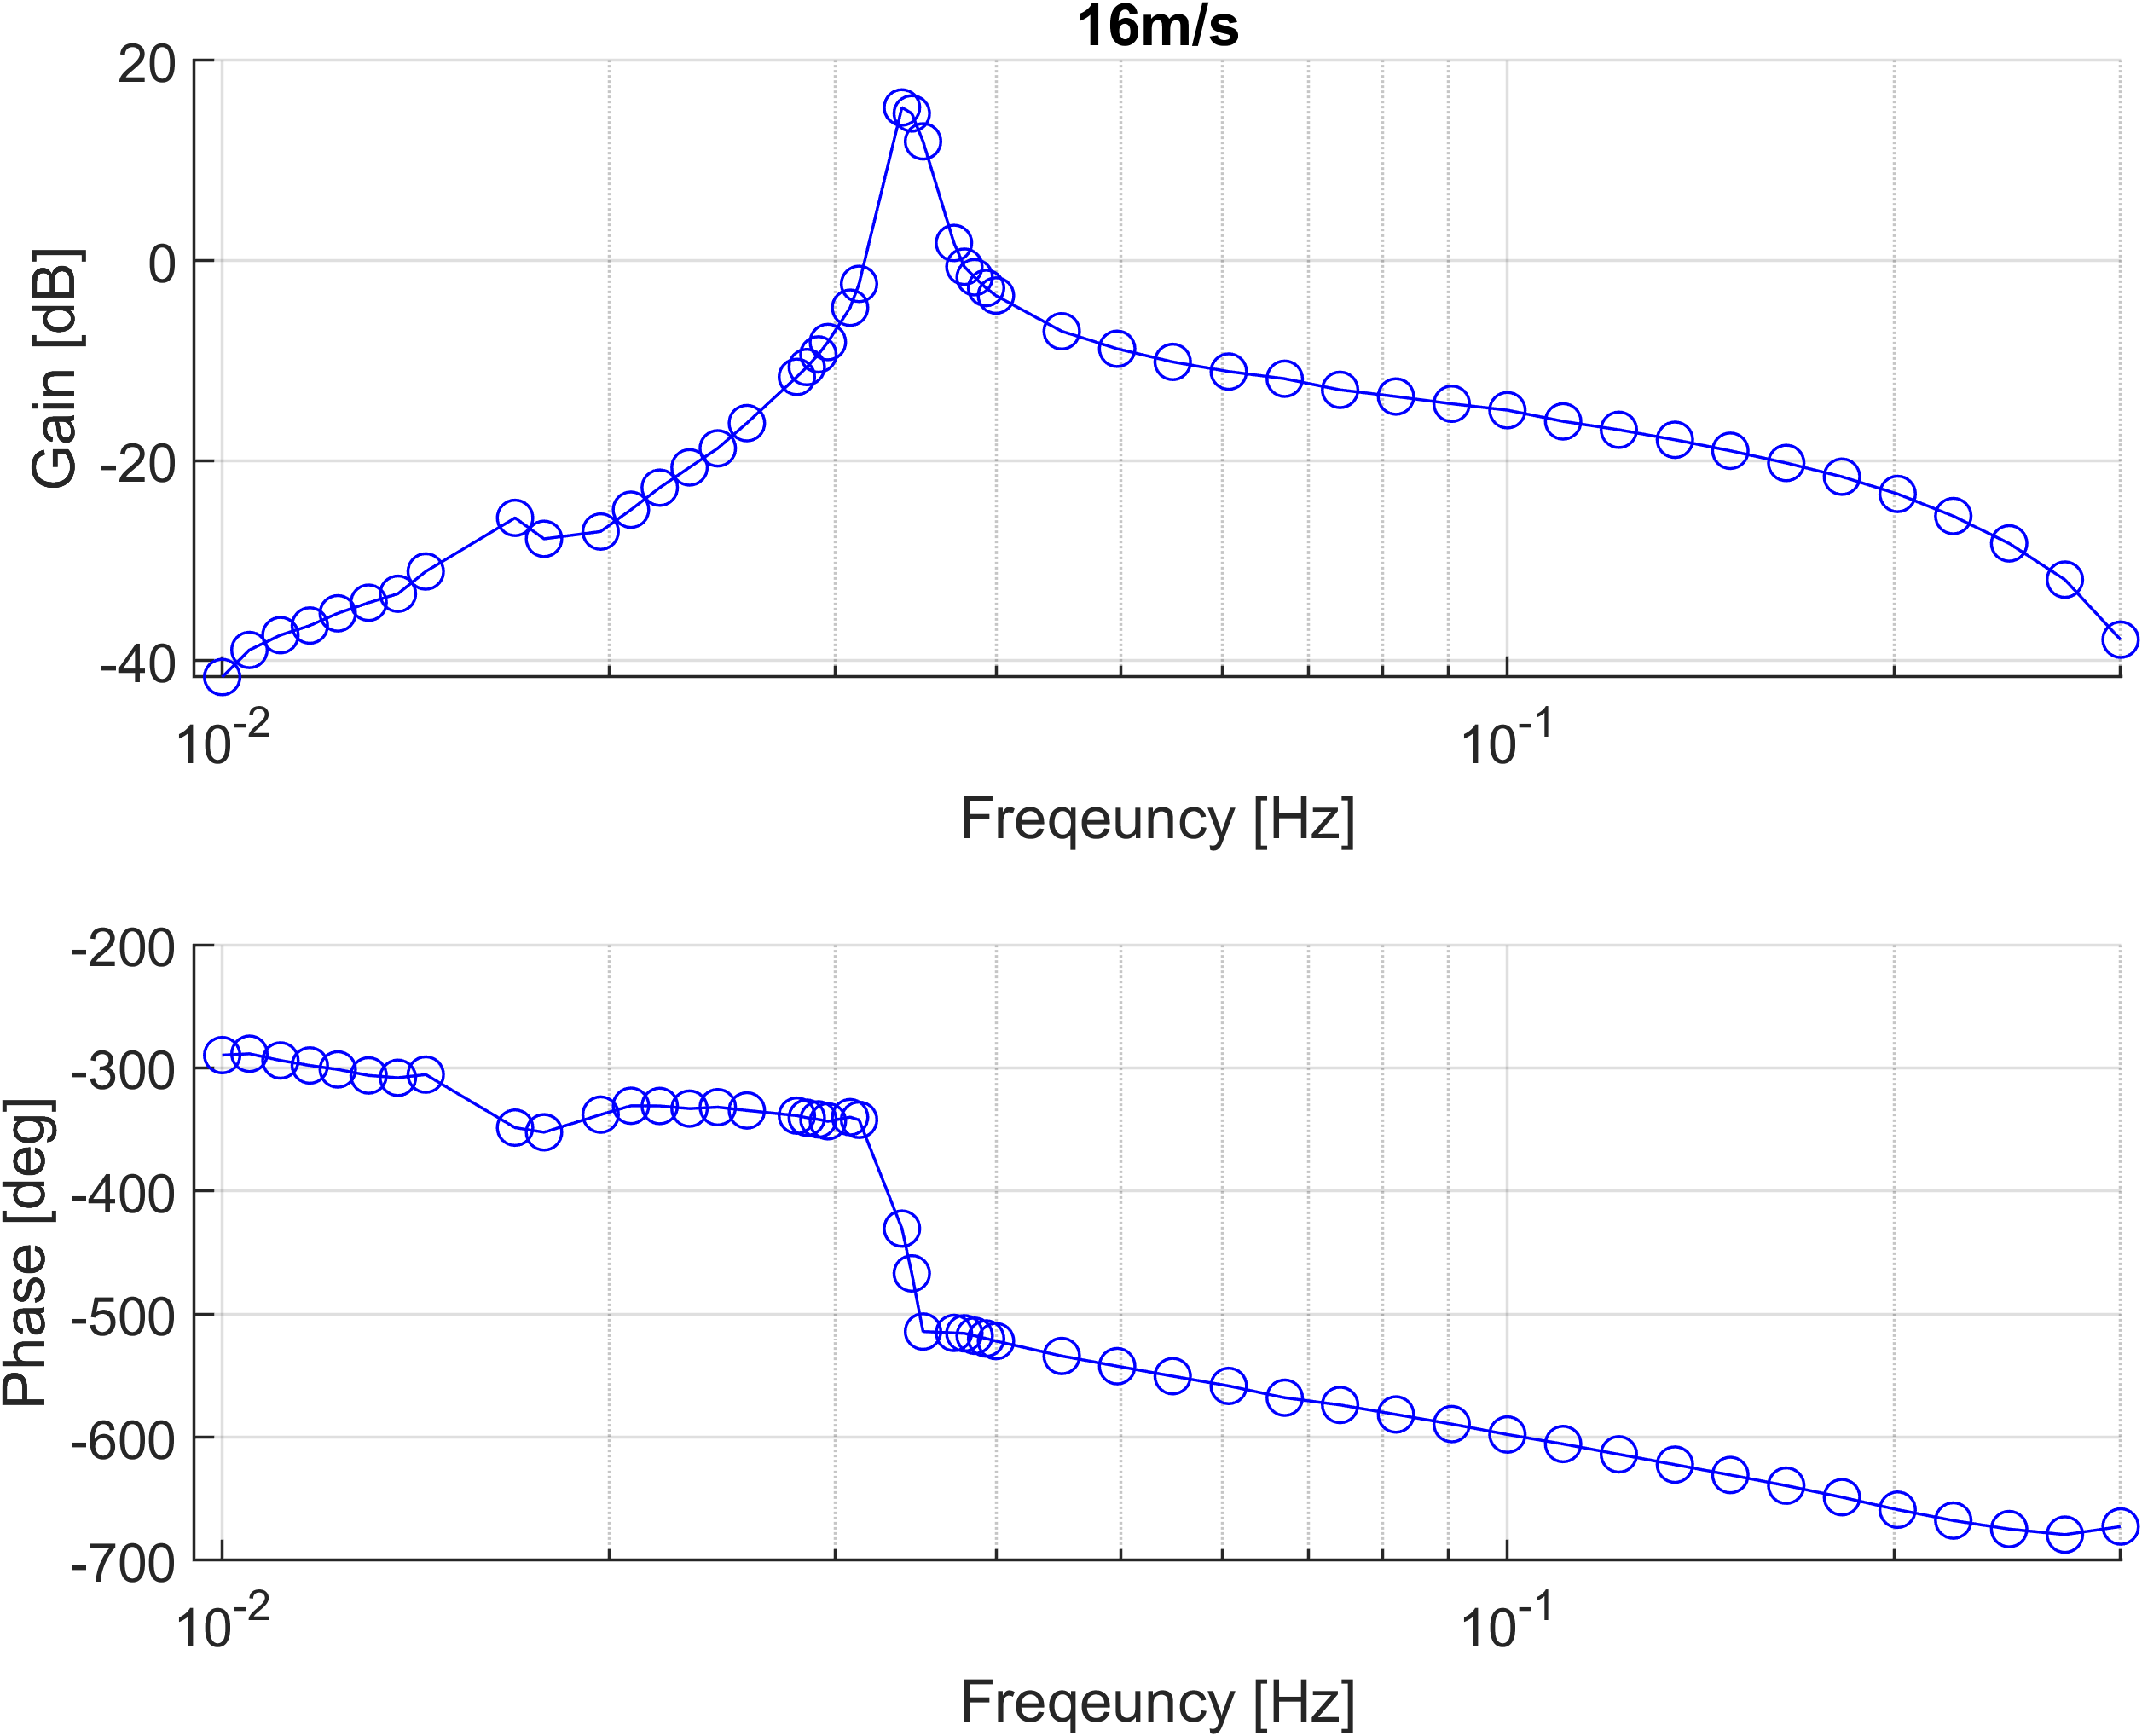
\includegraphics[width=.49\textwidth]{Graphics/TestResults/foreaftFitting/sysid_thSine-vy_16ms.png}
		\label{fig:app_sysid_thSine-vy_16}}
	\hfil
	\subfloat[Linear model response]{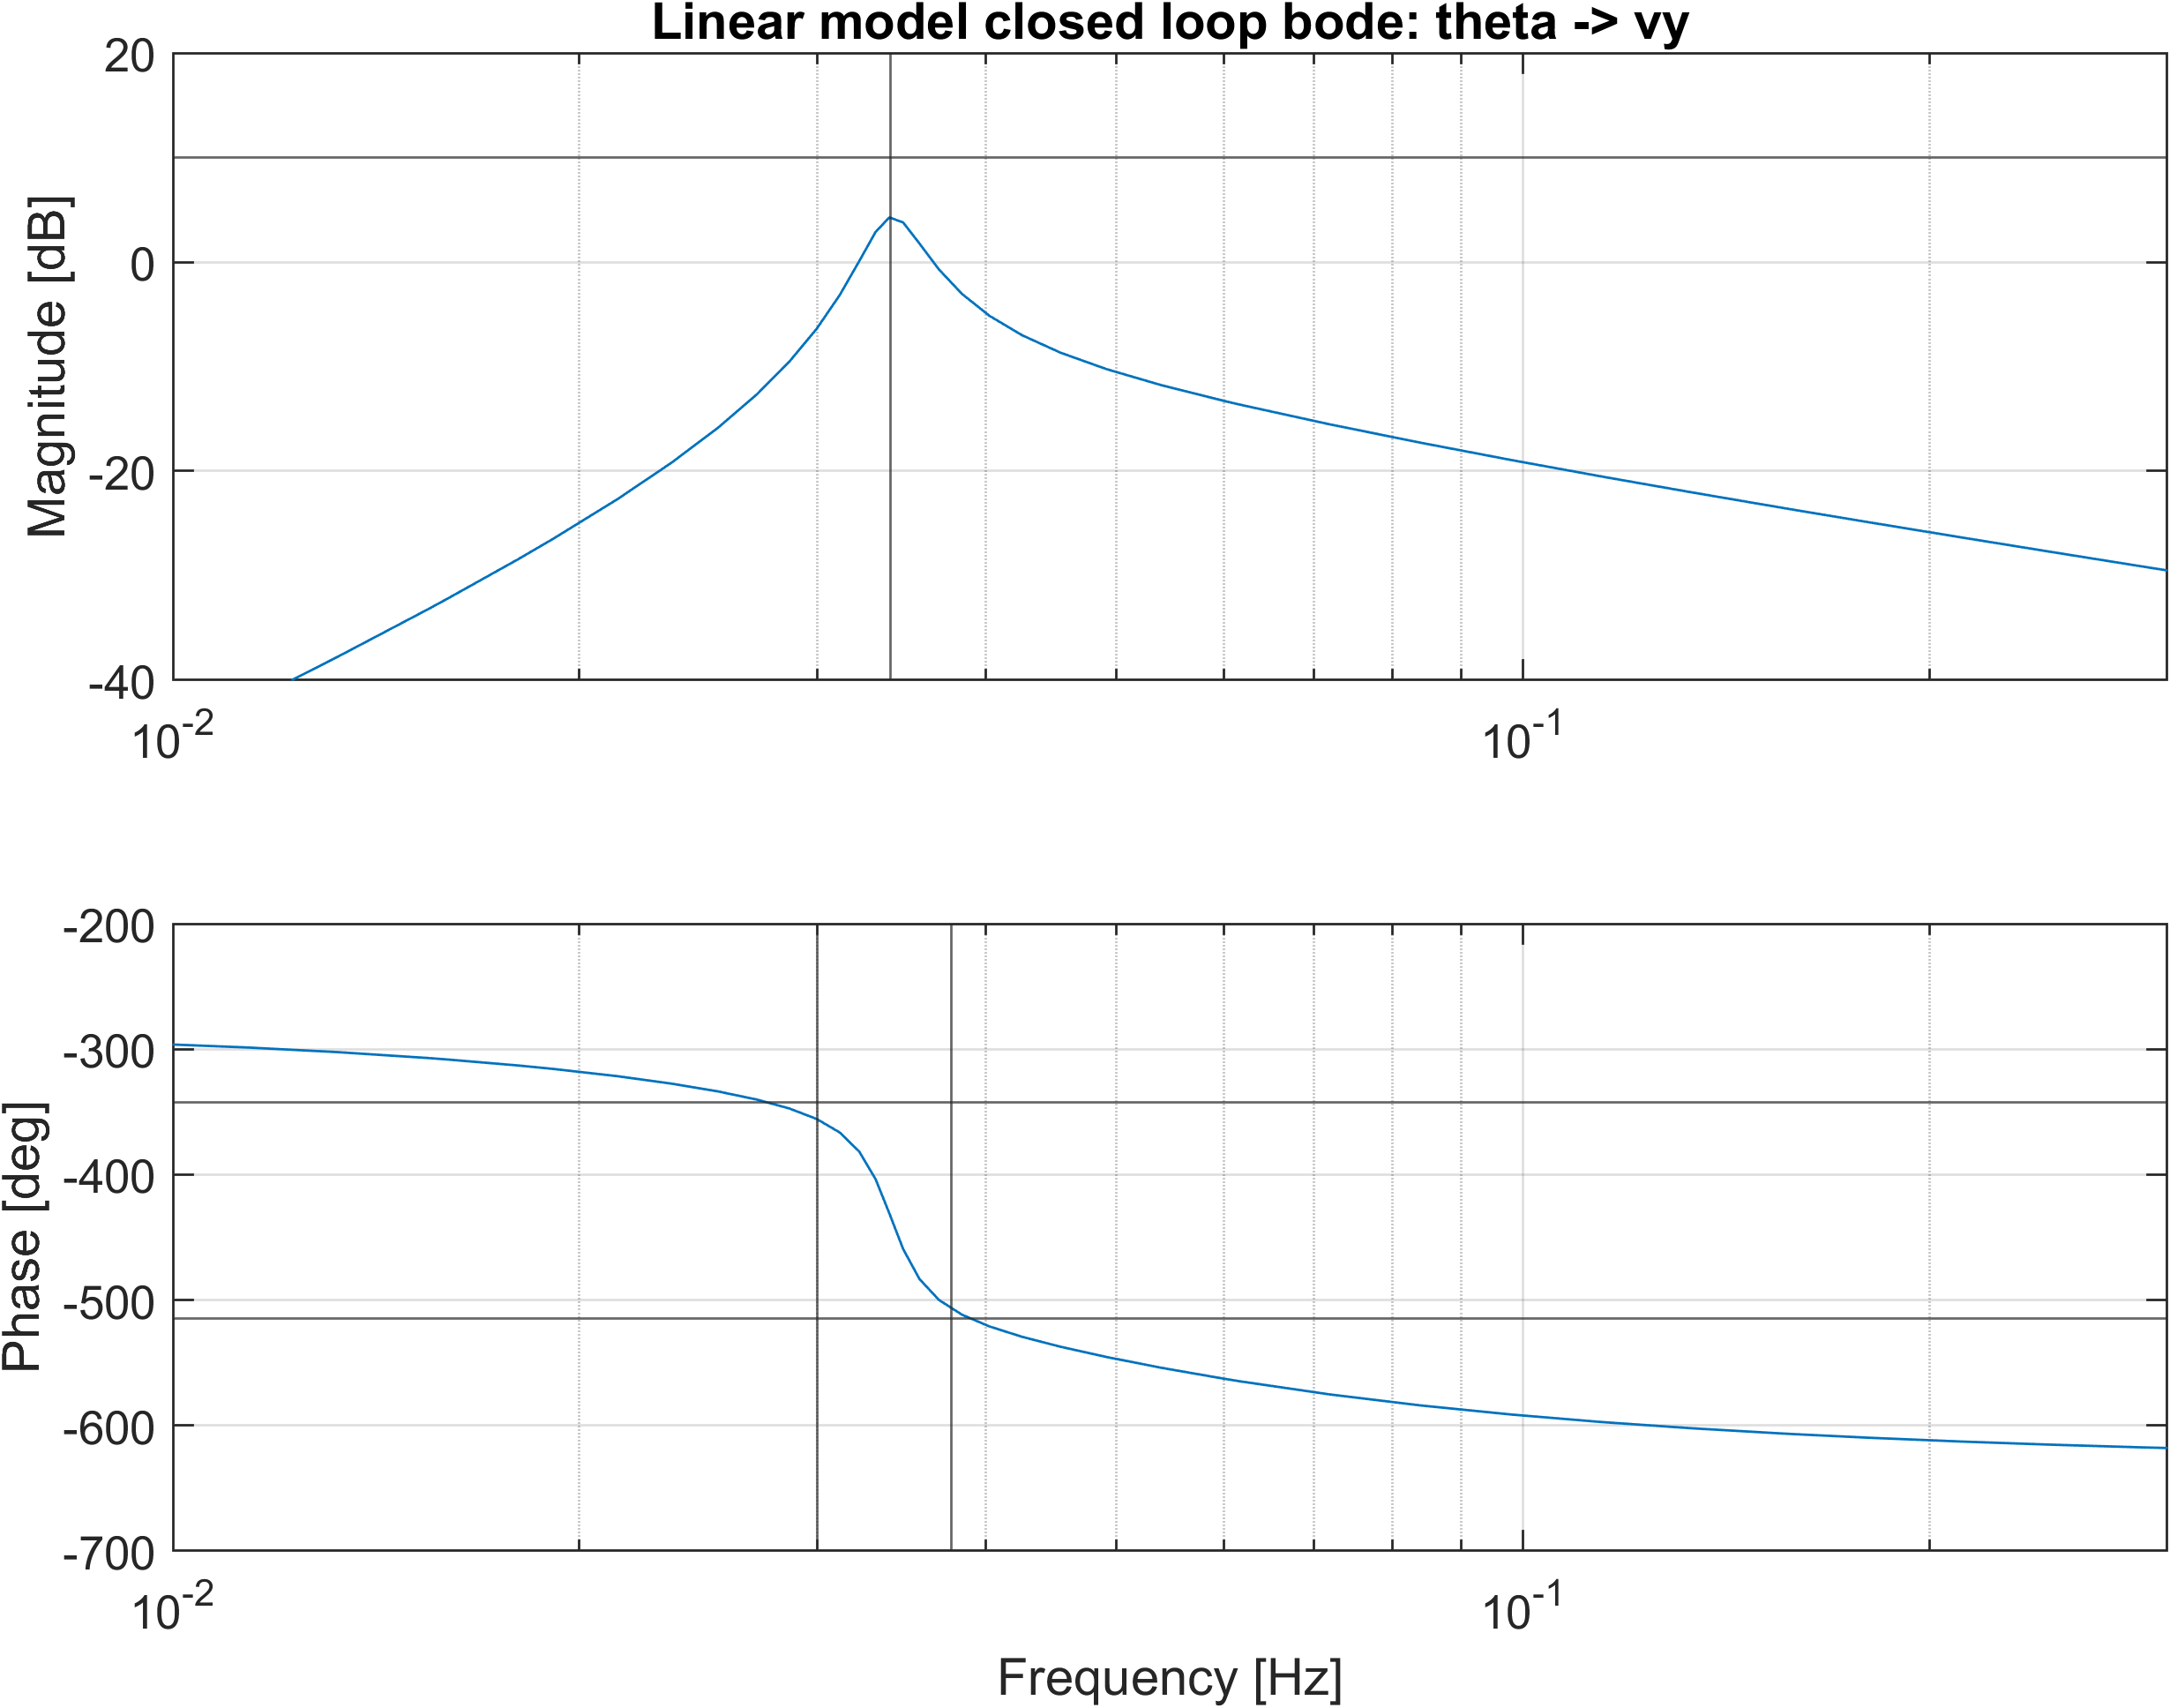
\includegraphics[width=.49\textwidth]{Graphics/TestResults/foreaftFitting/wtLin_th-vy_16ms.png}
		\label{fig:app_wtLin_th-vy_16}}
	
	\caption{pitch reference to fore-aft surge velocity fitting with operating point at 16 m/s; \textbf{(a)} VTS bode plot; \textbf{(b)} Linear model bode plot. Black lines are positioned in the magnitude plot to indicate the location of the peak of the VTS bode plot magnitude in (a). Black lines also indicate the position of the beginning and end of the large phase shift around the eigenfrequency from (a).}
	\label{fig:app_th-vy_16}
\end{figure*}



% Template
%\begin{figure*}[ht]
%	\centering
%	
%	\subfloat[VTS frequency response]
%	{\includegraphics[width=.49\textwidth]{Graphics/}%
%		\label{fig:app_sysid_}}
%	\hfil
%	\subfloat[Linear model response]
%	{\includegraphics[width=.50\textwidth]{Graphics/}%
%		\label{fig:app_wtlin_}}
%	
%	\caption{General_text; \textbf{(a)} a_text; \textbf{(b)} b_text.}
%	\label{fig:app_full}
%\end{figure*}


\subsection{Test: Linear model} \label{sec:app_test_lin}
The purpose of this test is to show and discuss the performance results of the LQI controller derived in \cref{sec:ctrl-design} on the linear model derived in \cref{sec:linear_model}. The controller is benchmarked against the original FLC controller with regards to both rotor speed control and fore-aft movement dampening capability. Prior to the test the LQI controller has been tuned such that a satisfactory performance was achieved in VTS.

It is expected that the LQI controller will perform much better in damping the fore-aft movement than the original FLC PI controller with no FATD. Test results are shown for both frequency and time domain.

% It is also expected to perform better in generator speed control despite the fact that the original FLC controller has been tuned to achieve the best possible generator speed tracking performance. The reason for this prediction might be less obvious. The reason is that the LQI controller has been tuned on the simple linear model and not in VTS like the FLC PI controller. Thus potential unforeseen consequences of having an aggressive controller in a more realistic environment are not discovered until it is tested in VTS.

\subsubsection{Test framework}
Matlab is used to makedf bode plots and Matlab Simulink is used to run time simulations. The Matlab \textit{connect()} function is utilized with component models defined on a specific form to gain transfer functions or state space systems from one or more inputs to one or more outputs. From these the \textit{bode()} Matlab function is used to make bode plots. 

Time simulations are made with the FLC PI and LQI controlled linear models from the $ A $, $ B $ and $ C $ system matrices and controller gains $ K $. In \cref{fig:app_simulink_setup2} the Simulink simulation setup is seen. Two systems are observed with the top one containing the original FLC PI controller without FATD enabled and the bottom one being the one with the designed LQI controller. While not directly apparent because of the missing state feedback, the top system is a closed loop system with the controller gain $ K $ contained in the $ A $ and $ B $ matrix. The reason for this is simply that the FLC component described in \cref{sec:comp_flc} is defined as a generic component model and conveniently combined with the Matlab \textit{connect()} function to yield a full closed-loop system.

From the left the free wind disturbance deviation from the OP is observed entering both systems. The wind data is extracted from VTS simulations and thus mimic the wind turbulence realistically. The simulation is run for a total of 1000 seconds and the states are initialized at the OP except for the tower top position $ p_y $ which is initialized with a deviation of 5 m to provoke a response from both systems.
\begin{figure}[ht]
	\centering
	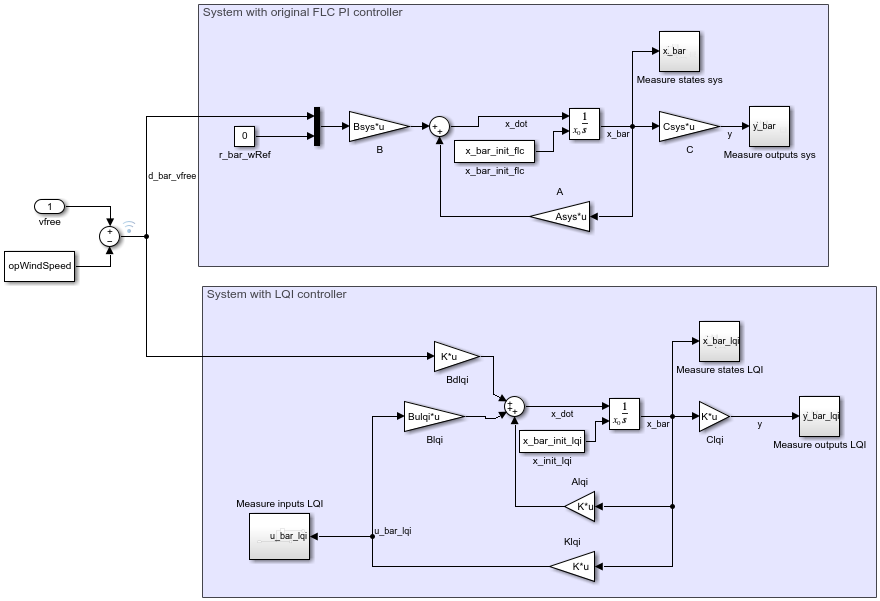
\includegraphics[width=0.95\linewidth]{Graphics/TestResults/linearModPerf/simulink_setup2.png}
	\caption{The Matlab Simulink setup. The free wind speed is observed entering the system from the left.}
	\label{fig:app_simulink_setup2}
\end{figure}


\subsubsection{Frequency Domain}
In figure \cref{fig:app_script_vfreeTovy} the frequency response from the free wind disturbance $ v_{free} $ to the fore-aft tower top velocity $ v_y $ is seen. Both the FLC PI system and LQI system are plotted for comparison. It is observed that the LQI controller yields much greater dampening of the eigenfrequency than the FLC PI controller.
\begin{figure}[ht]
	\centering
	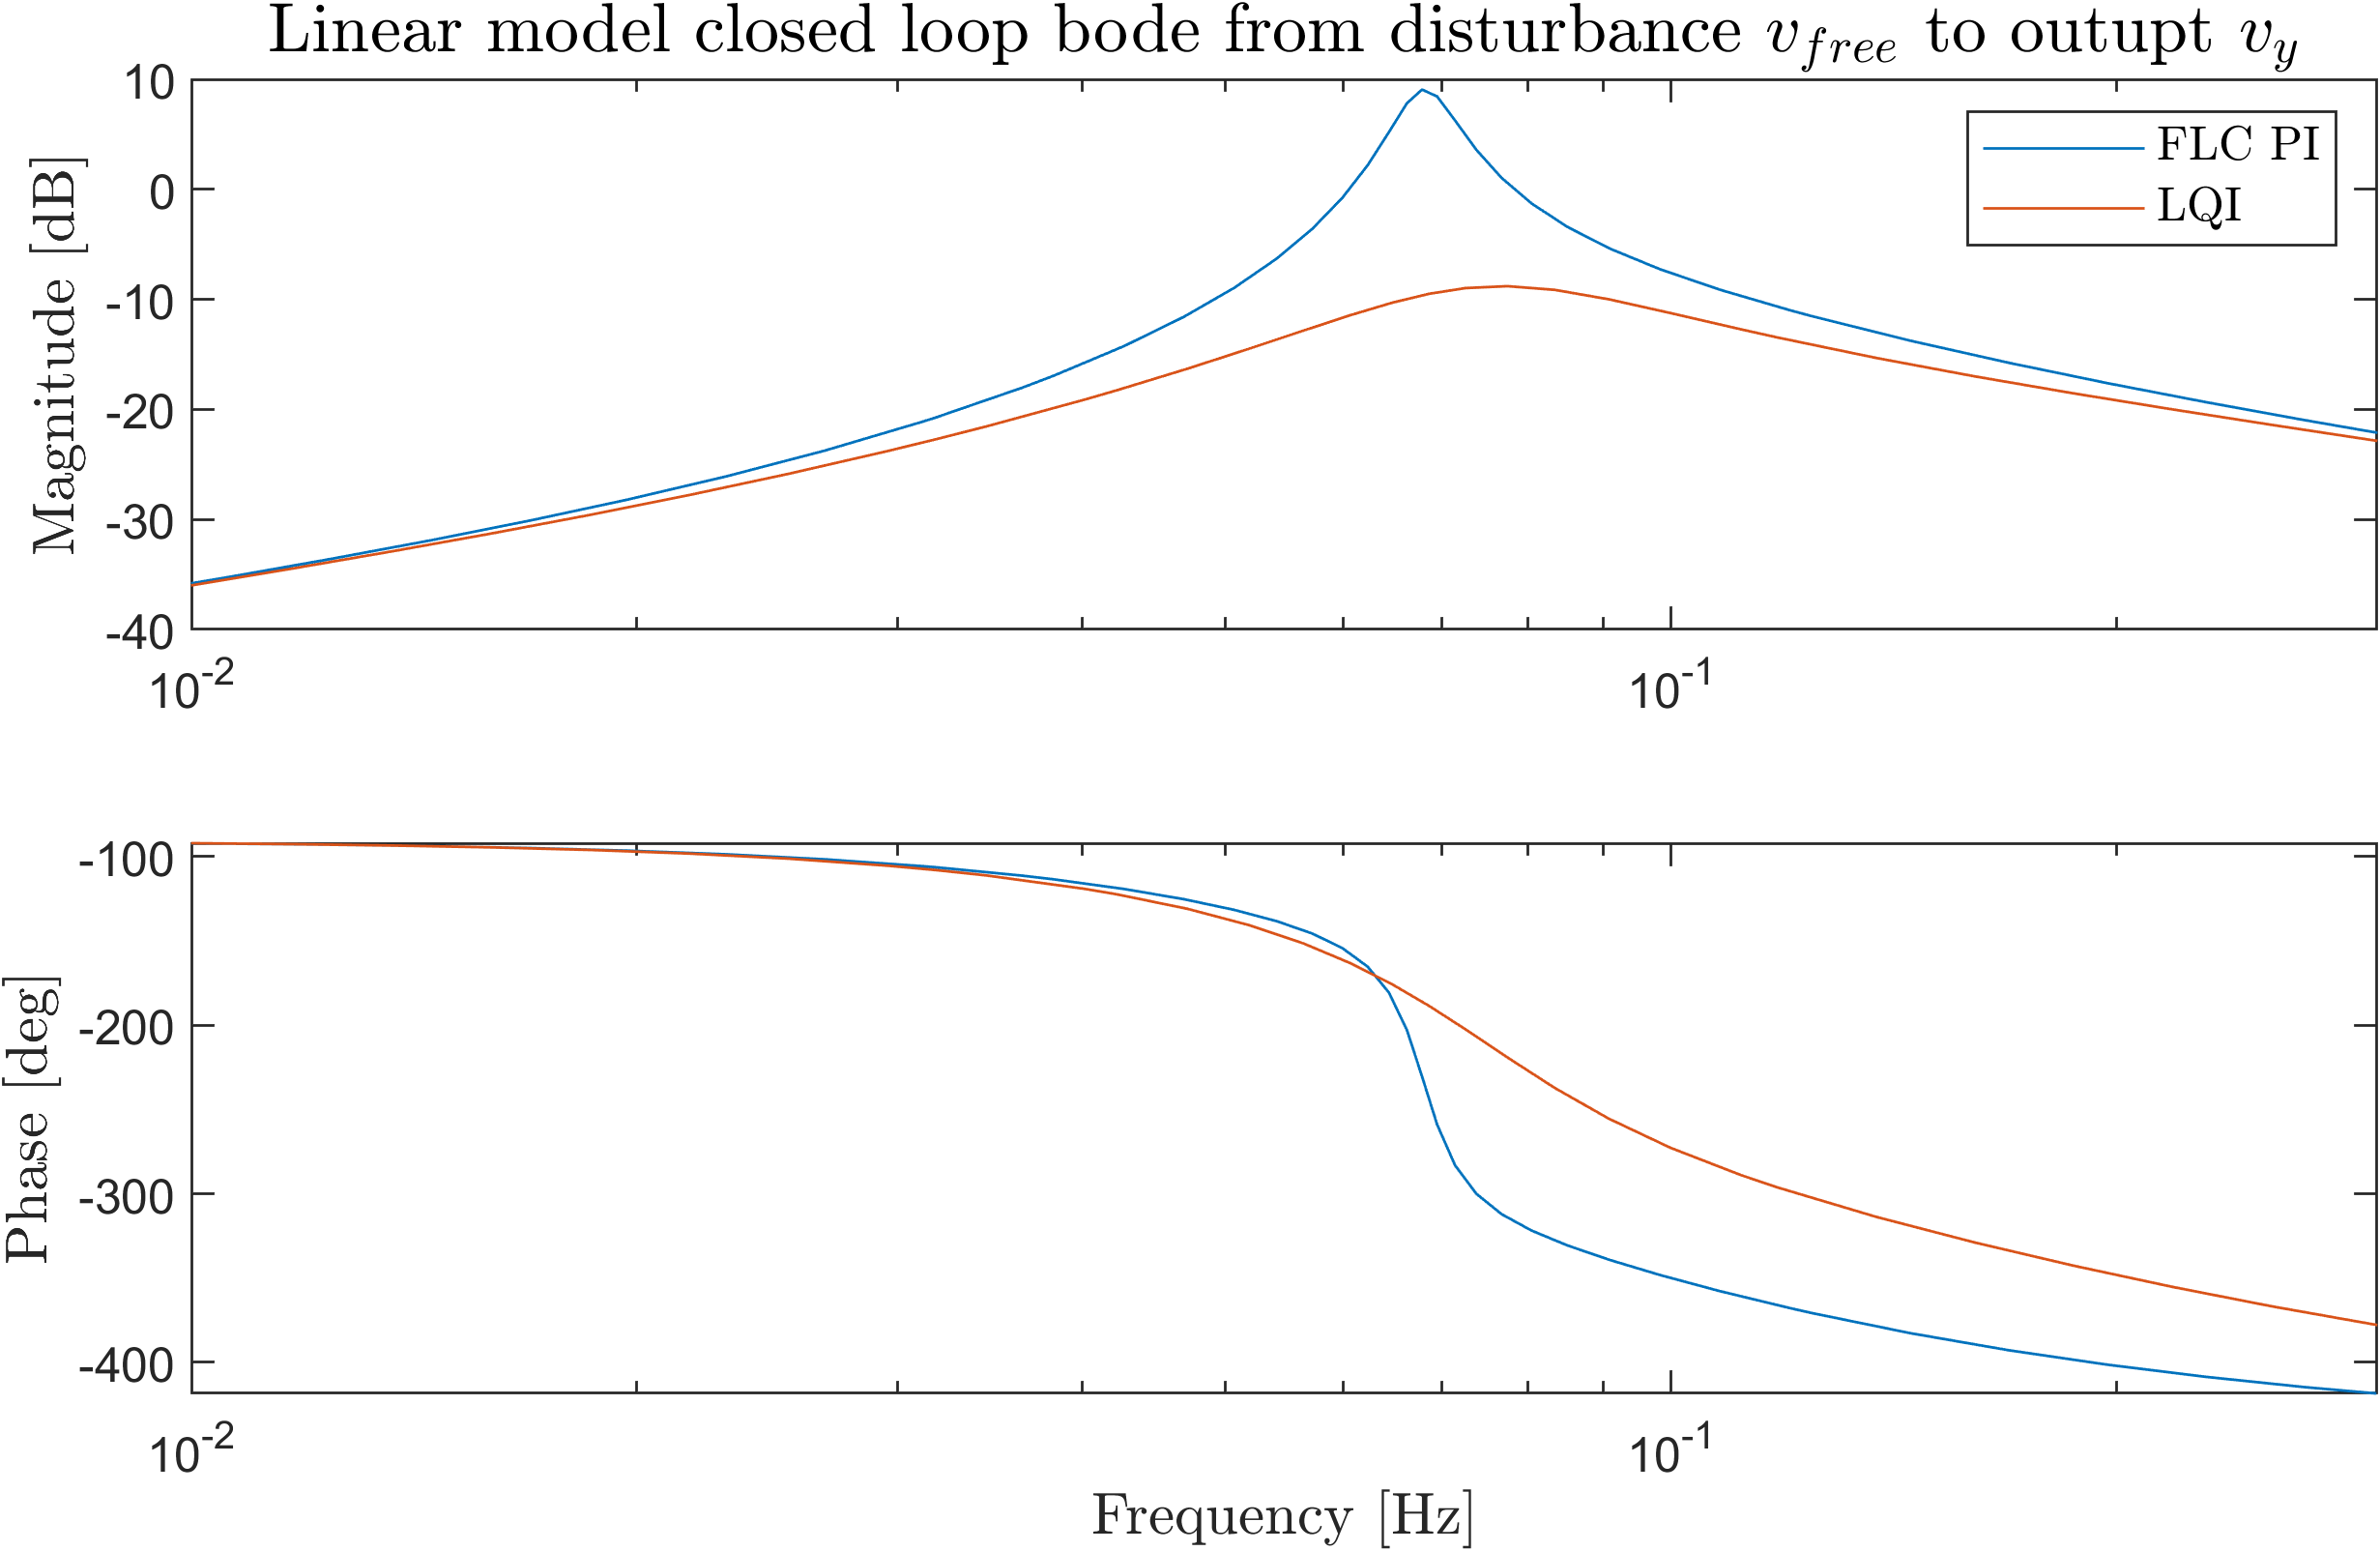
\includegraphics[width=0.7\linewidth]{Graphics/TestResults/linearModPerf/script_vfreeTovy.png}
	\caption{Frequency response from the free wind as observed by the rotor ($ v_{free} $) to the fore-aft velocity ($ v_y $) of the linear model with a comparison between the original FLC PI controller and the LQI controller.}
	\label{fig:app_script_vfreeTovy}
\end{figure}
In \cref{fig:app_script_vfreeTovy} where the frequency response from $ v_{free} $ to $ \Omega $ is plotted the same tendency is observed. The LQI controller furthermore dampens the magintude around 4-7 dB more than the FLC PI controller before the eigenfrequency around 0.035 Hz. It also dampens the magnitude more after the eigenfrequency but decreasingly for higher frequencies.
\begin{figure}[ht]
	\centering
	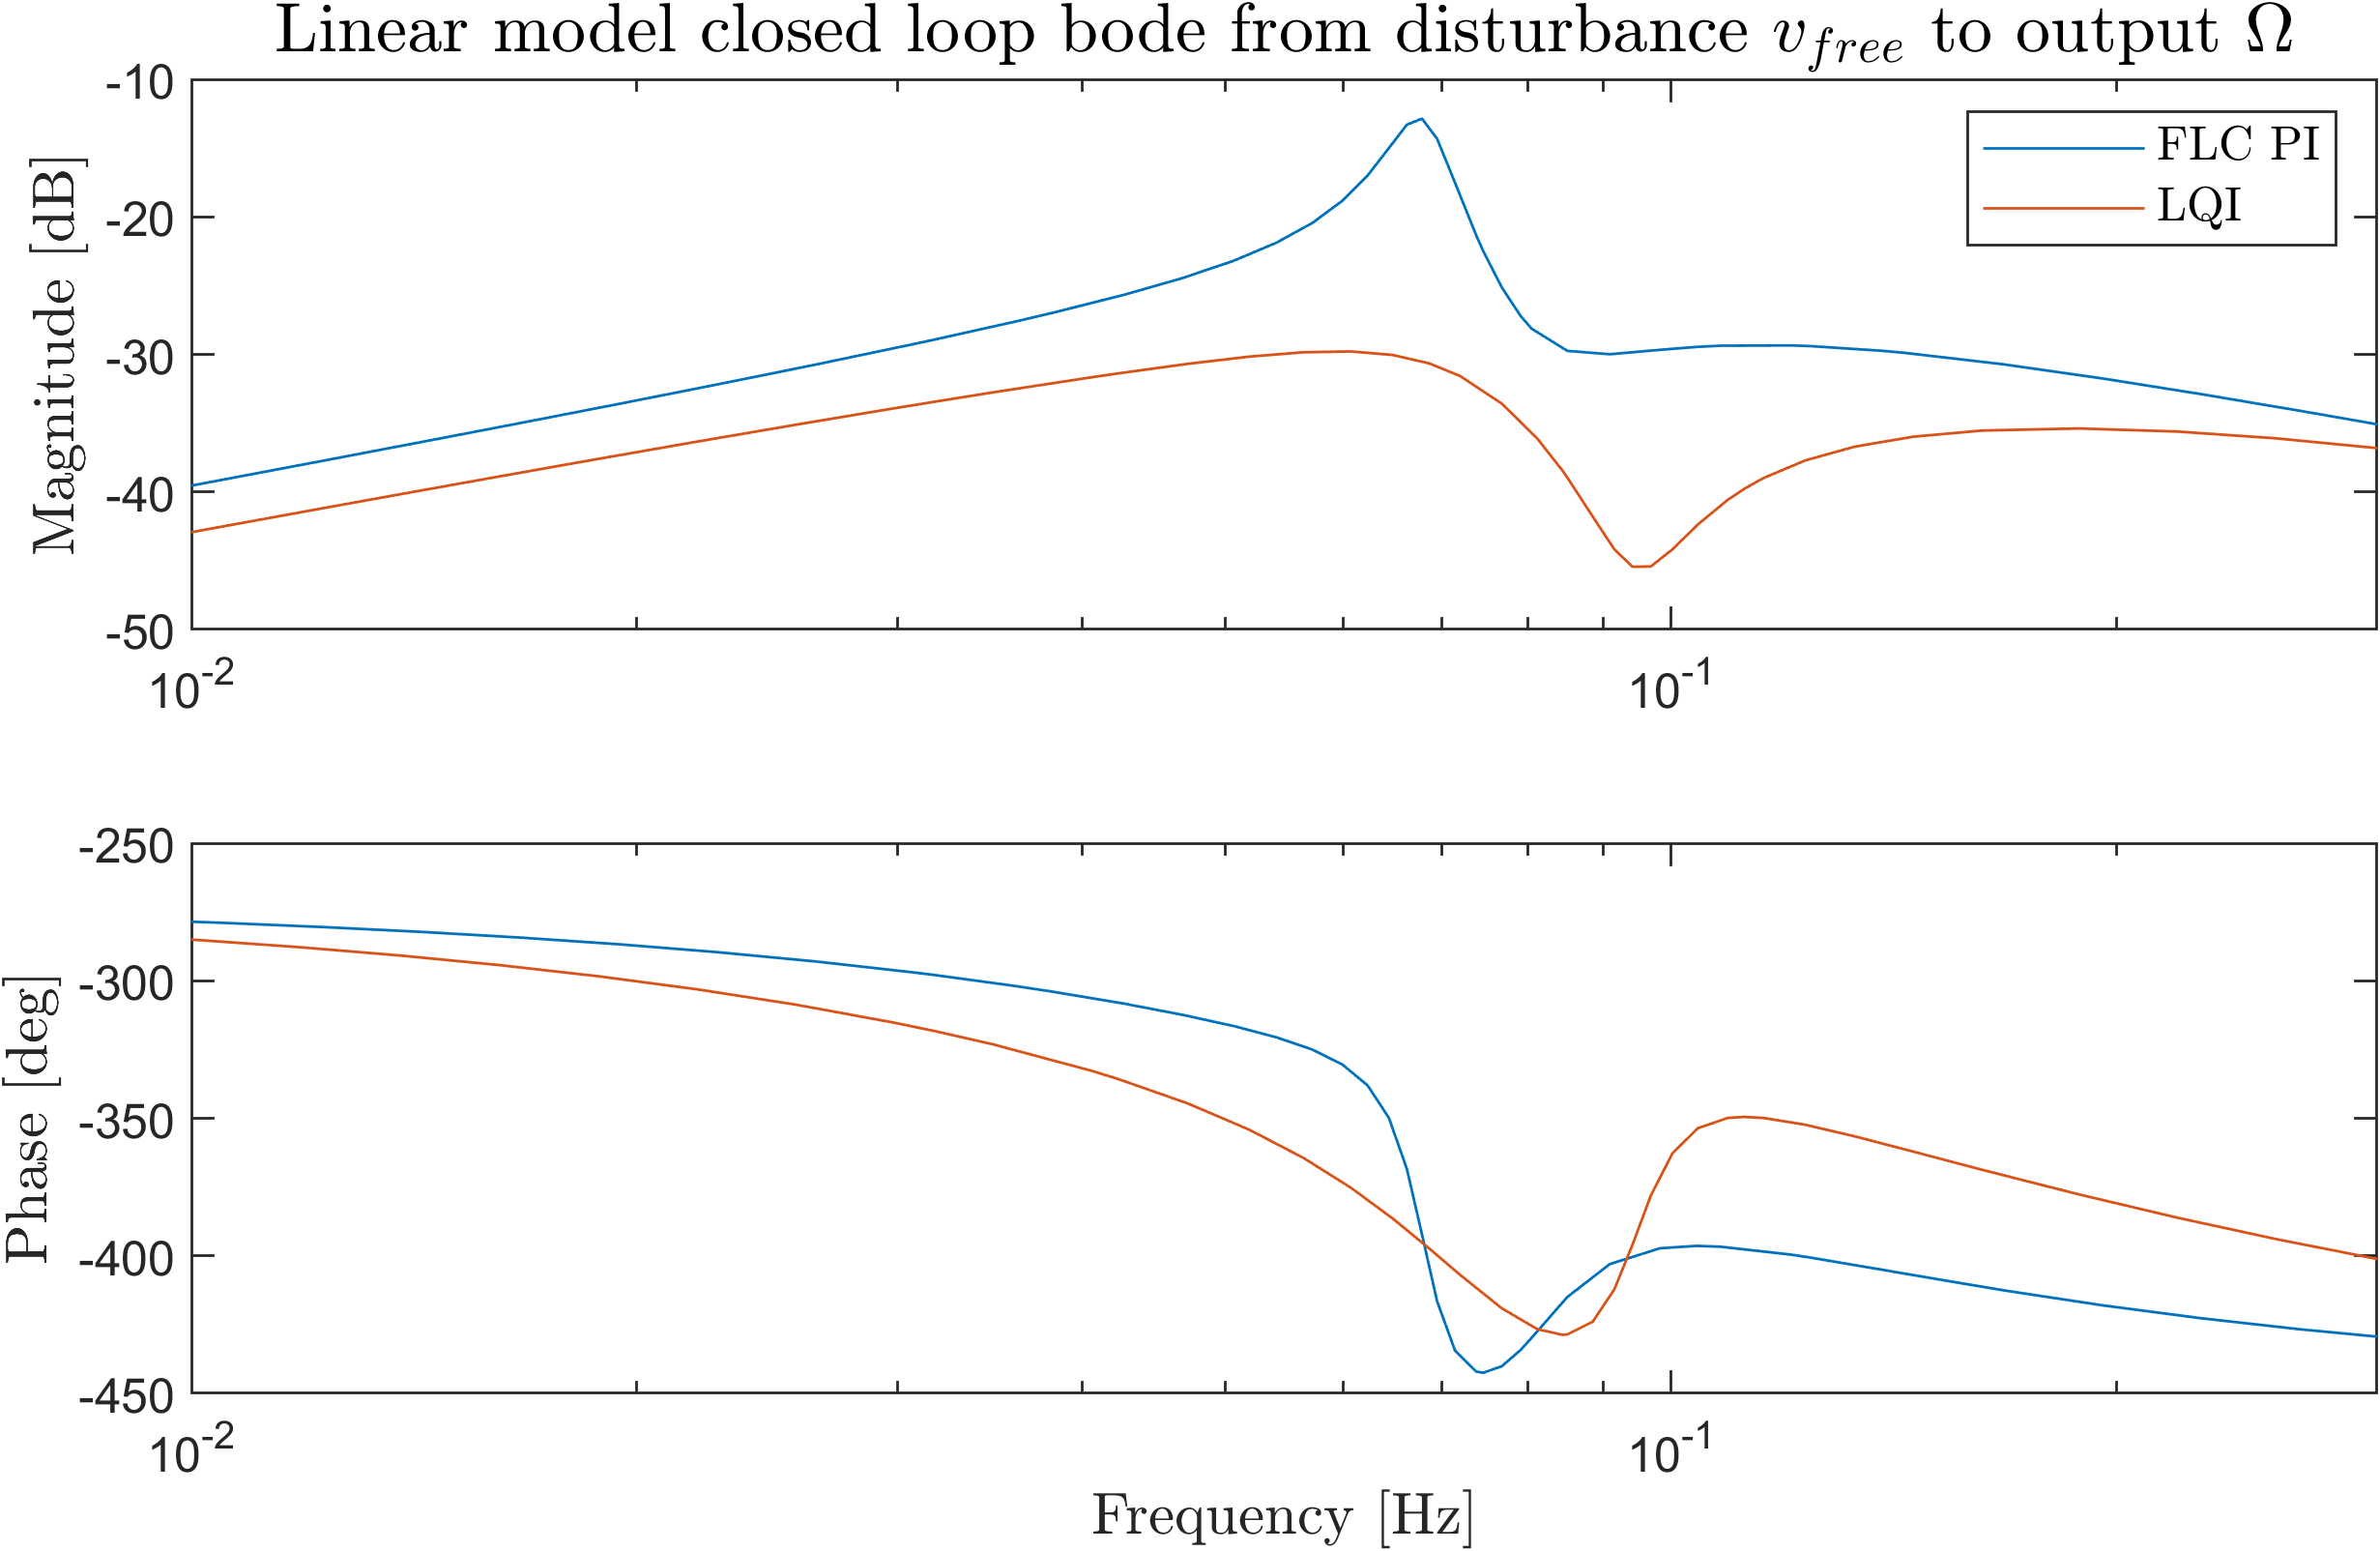
\includegraphics[width=0.7\linewidth]{Graphics/TestResults/linearModPerf/script_vfreeToW.png}
	\caption{Frequency response from the free wind as observed by the rotor ($ v_{free} $) to the rotor speed ($ \Omega $) of the linear model with a comparison between the original FLC PI controller and the LQI controller}
	\label{fig:app_script_vfreeToW}
\end{figure}
From the frequency responses it can be concluded that the LQI controller will perform better at both rotor speed tracking and fore-aft movement damping. 

\clearpage
\subsubsection{Time domain}
In \cref{fig:app_sim_11_W_py_vy_comp} the rotor speed, fore-aft position and fore-aft velocity is plotted. Both the FLC PI and LQI controlled systems are plotted for comparison. Both rotor speed tracking and fore-aft motion performance is vastly superior for the LQI controller. The poor rotor speed tracking performance of the FLC controller is expected because of its lack of consideration for the fore-aft motion.
\begin{figure}[ht]
	\centering
	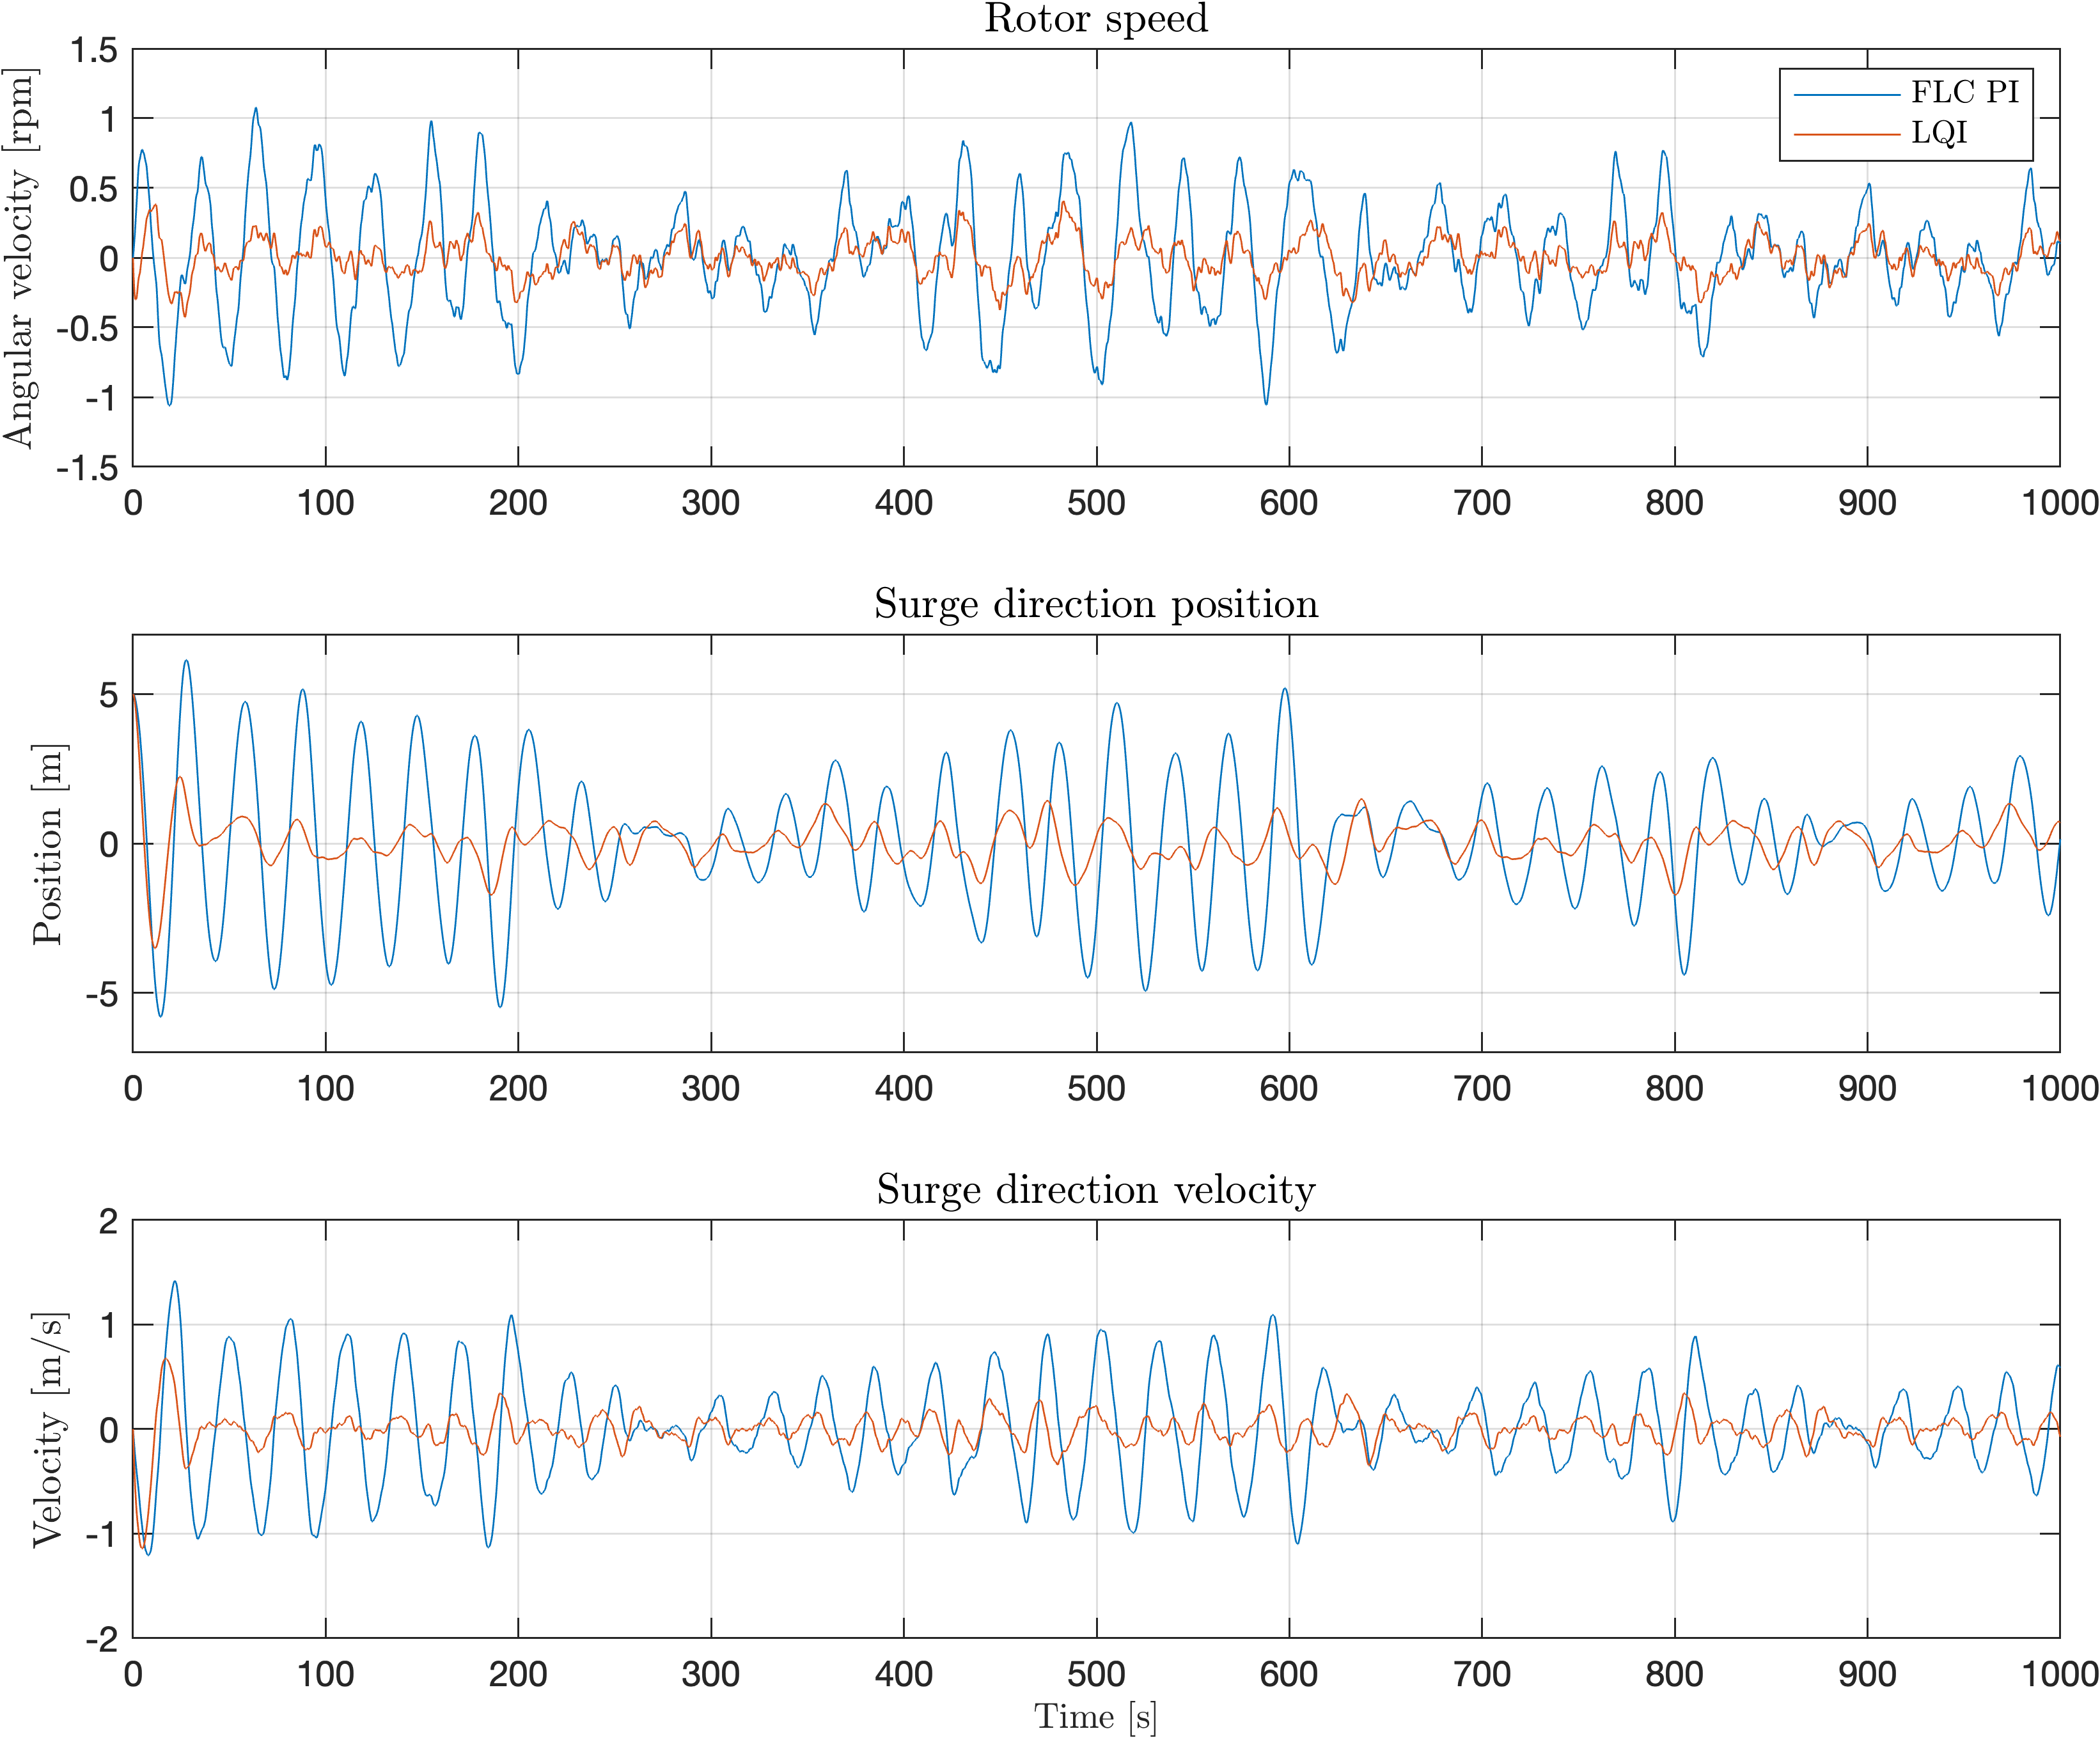
\includegraphics[width=0.7\linewidth]{Graphics/TestResults/linearModPerf/sim_11_W_py_vy_comp.png}
	\caption{Simulink simulation results. The 5 m deviation initialization of the tower top position is visible from the \textit{fore-aft position} at 0 s.}
	\label{fig:app_sim_11_W_py_vy_comp}
\end{figure}
\cref{fig:app_sim_12_W_py_vy_comp_zoom} shows a plot zoomed in at the start of the simulation. It is apparent that the LQI controller corrects for the fore-aft position deviation effectively in 30 to 40 seconds.
\begin{figure}[ht]
	\centering
	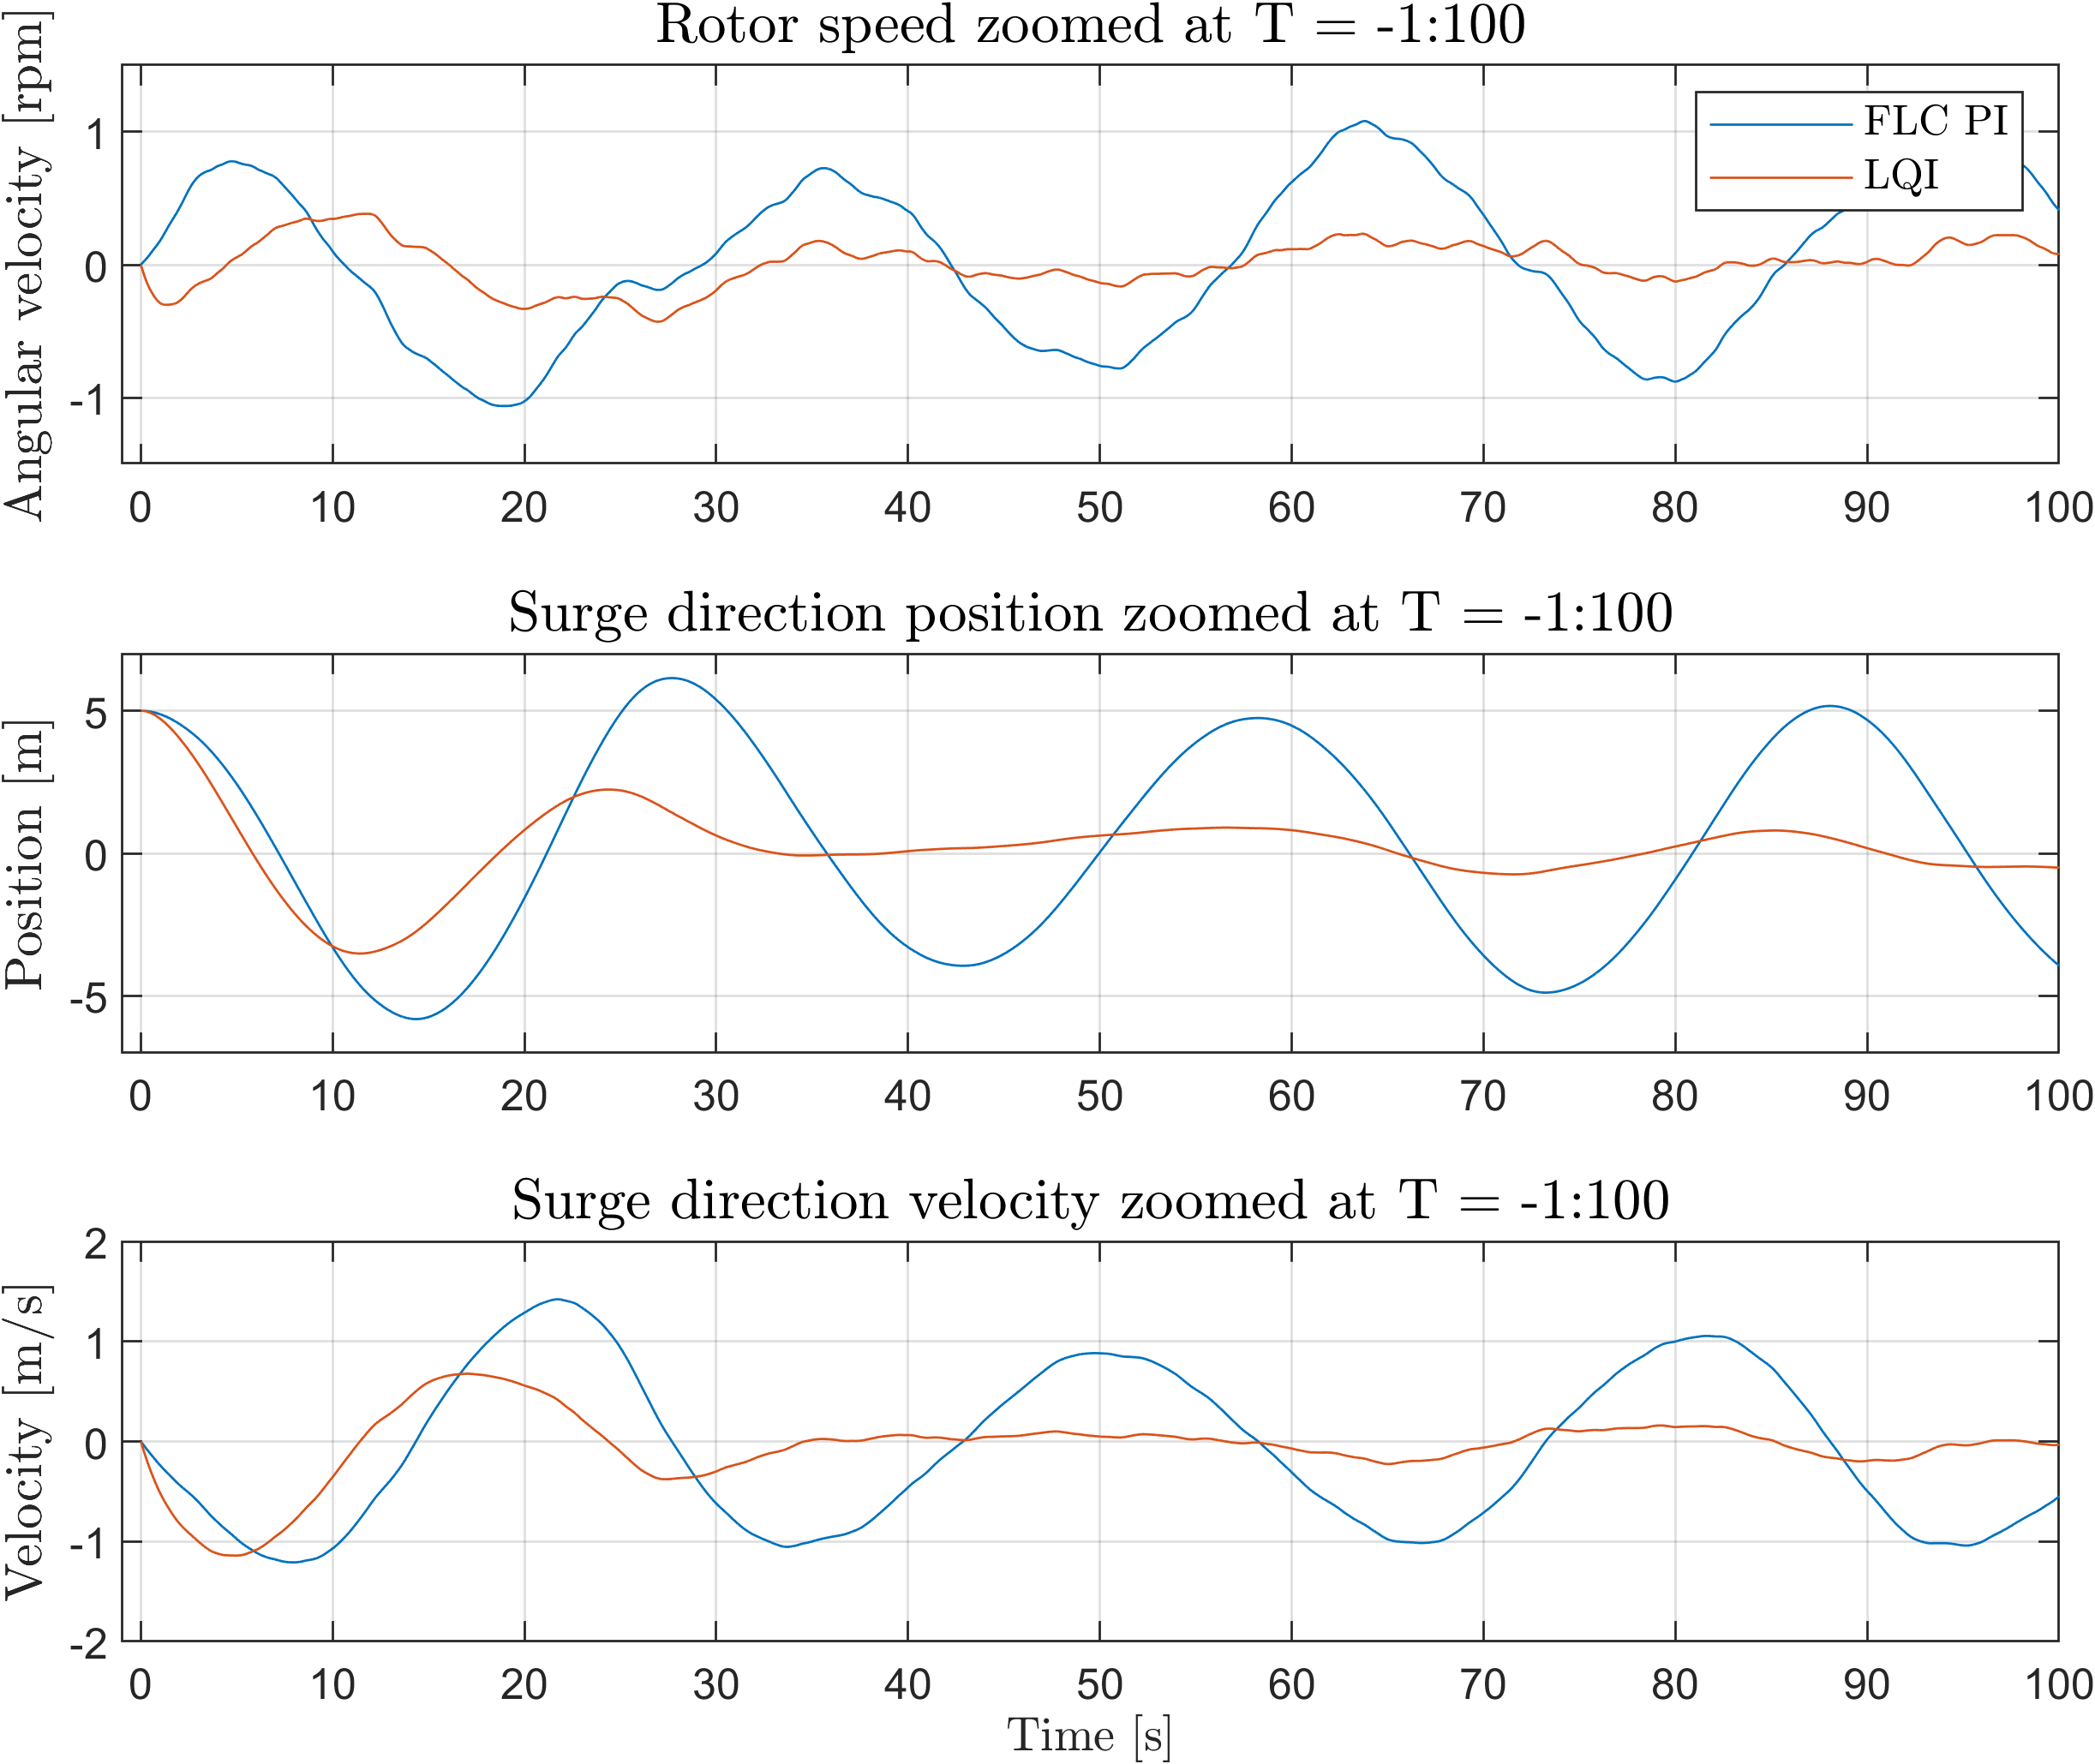
\includegraphics[width=0.7\linewidth]{Graphics/TestResults/linearModPerf/sim_12_W_py_vy_comp_zoom.png}
	\caption{Simulink simulation results zoomed in at the first 100 seconds where the fore-aft position is initialized at 5 m.}
	\label{fig:app_sim_12_W_py_vy_comp_zoom}
\end{figure}

The LQI controller pitch reference deviation from the OP and its rate of change is plotted in \cref{fig:app_sim_10_pitch}. Both the absolute value of the pitch reference and its rate of change should not exceed values which are realistic for the wind turbine at the OP. Simulations of the turbine in VTS has shown that a blade pitch rate of change of 2 deg/s and an absolute pitch deviation from the OP of 3-4 is fairly common. In the initial transient where the fore-aft position deviates by 5 m the pitch reference starts at 6 degrees and decreases with a rate og change starting at close to -3 deg/s. Neither the rate of change nor the absolute value are deemed problematic especially because such an abrupt change would not occur in a realistic scenario. For the remainder of the simulation the absolute value of the pitch reference deviation stays below 4 deg and the rate of change absolute value stays below 2 deg/s. These values are well inside an acceptable range.
\begin{figure}[ht]
	\centering
	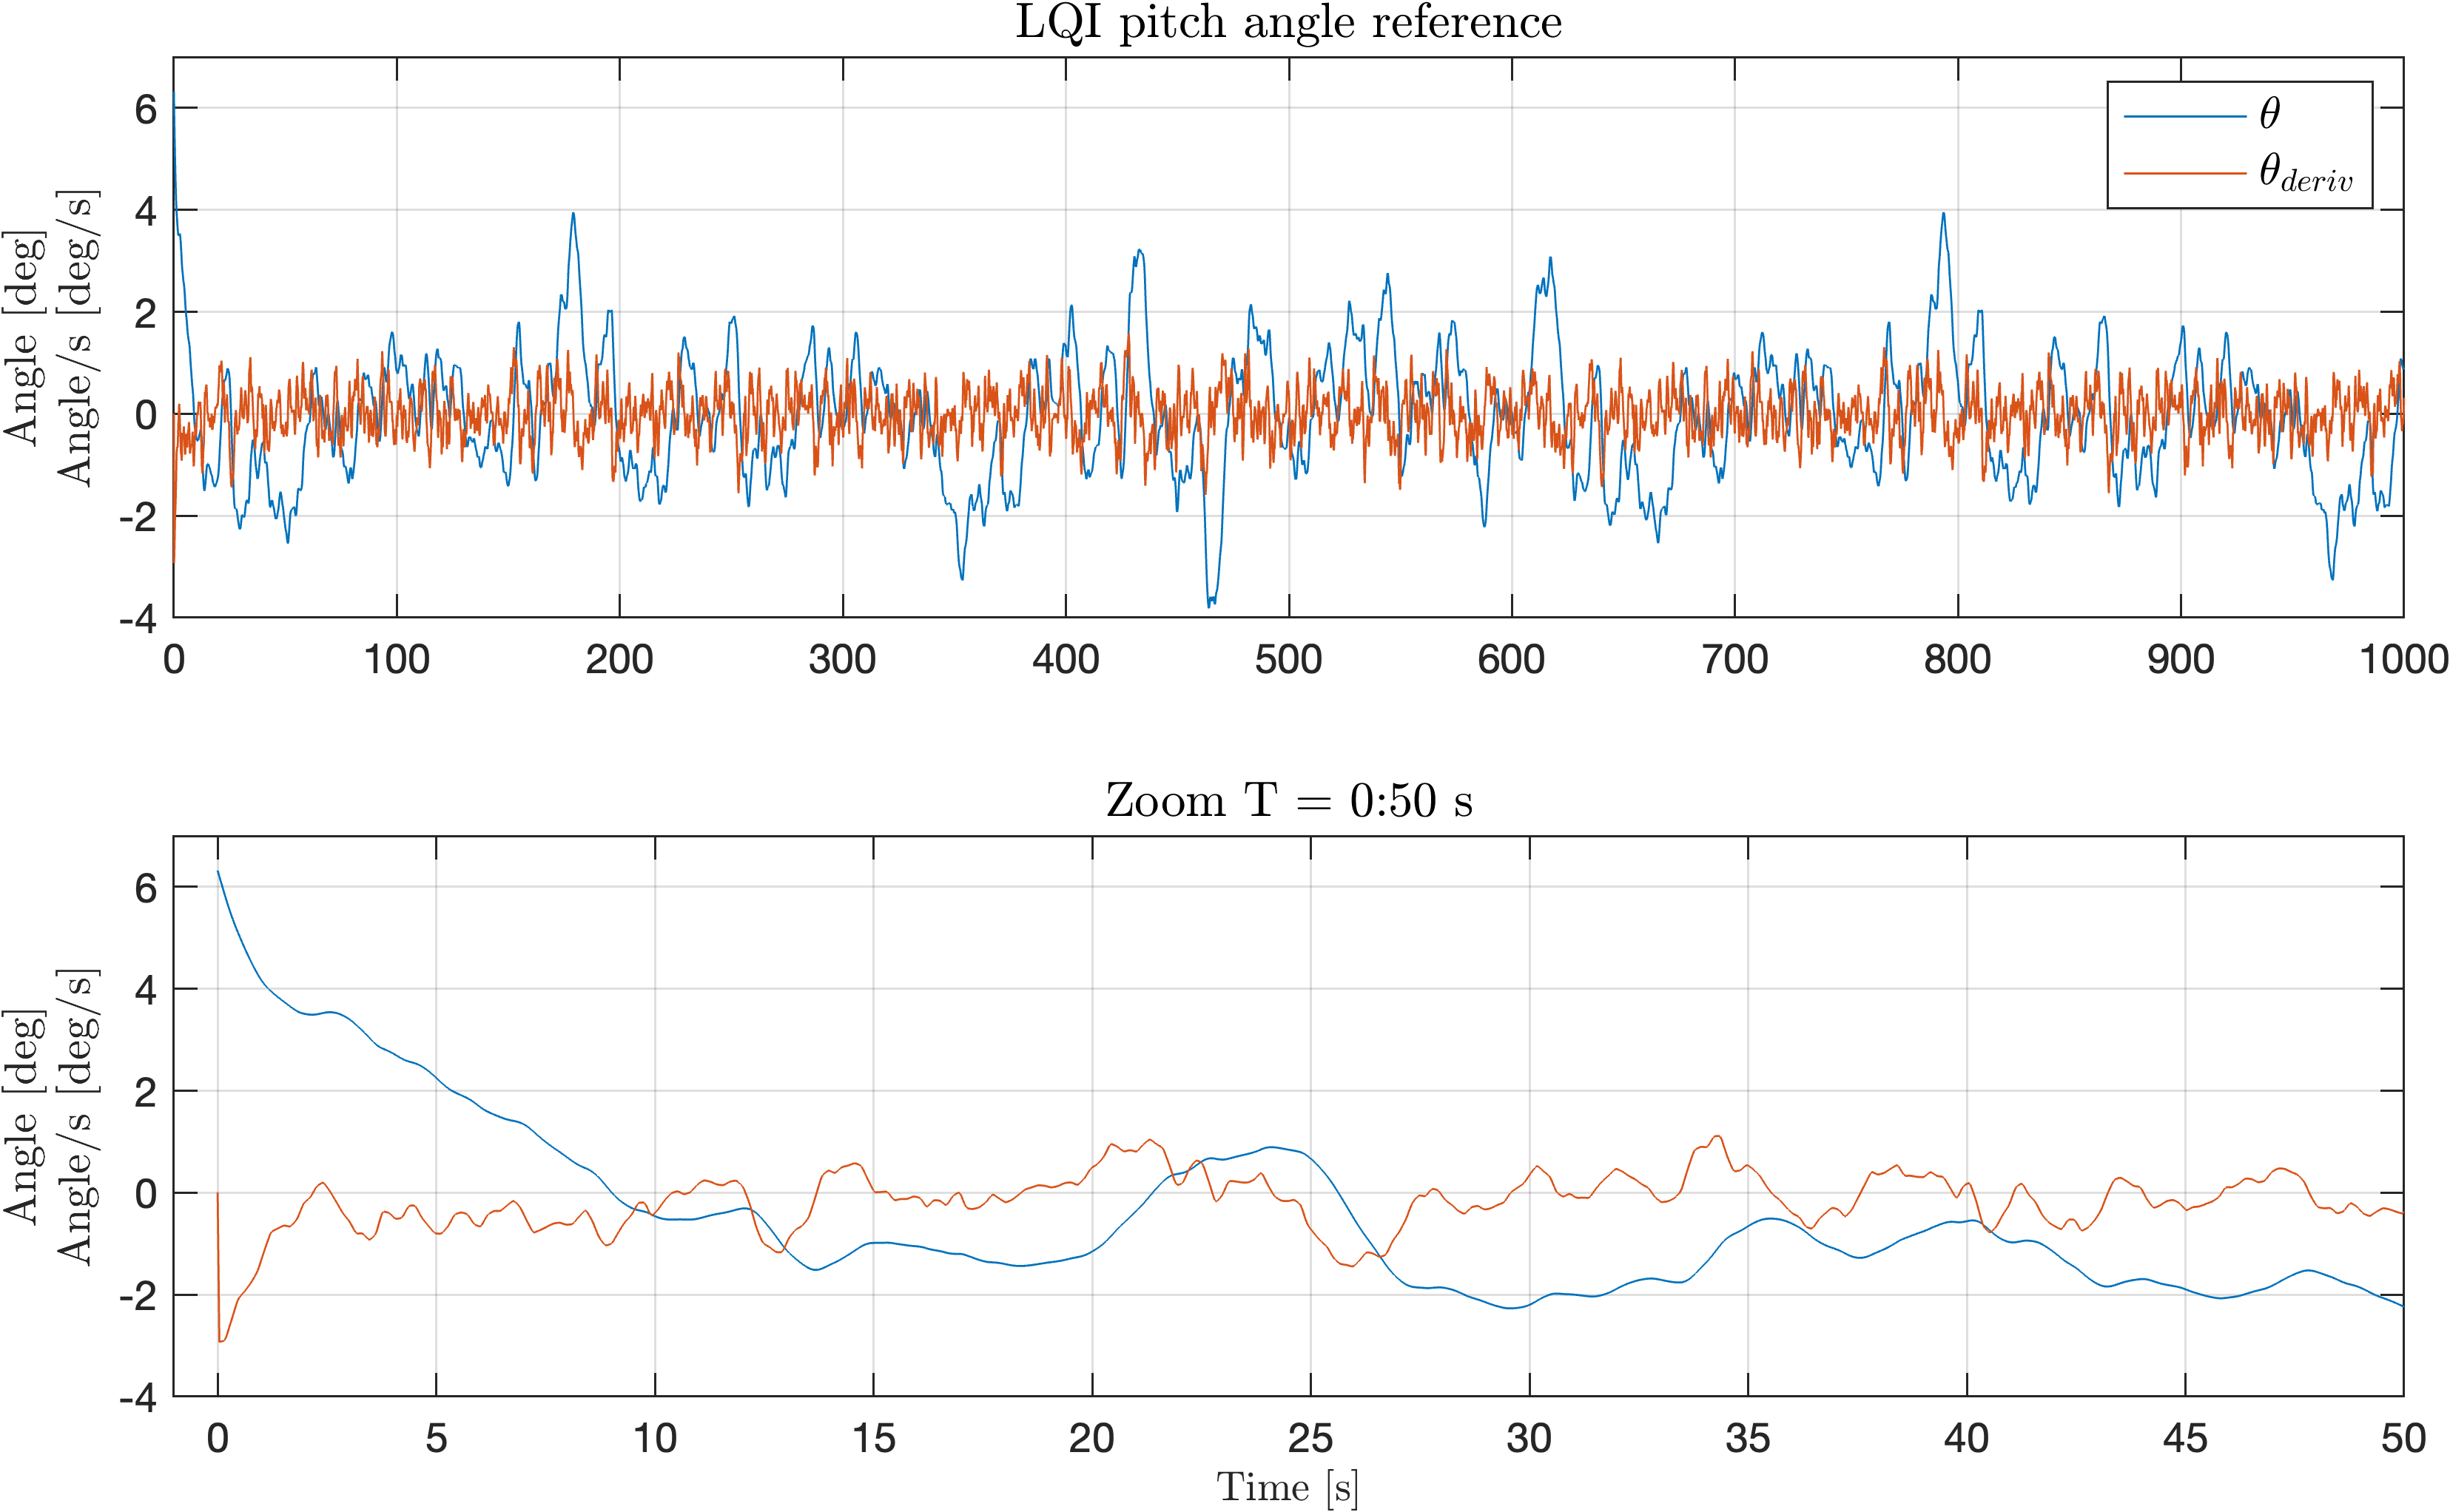
\includegraphics[width=0.7\linewidth]{Graphics/TestResults/linearModPerf/sim_10_pitch.png}
	\caption{Simulink simulation results of the pitch reference and pitch reference change. Neither the absolute value of the pitch reference nor the change in pitch reference reach alarming values.}
	\label{fig:app_sim_10_pitch}
\end{figure}

Conclusively the LQI controller performance is very good on the linear model in comparison to the FLC PI controller.% This is also to be expected given the...


% OLD PLOTS WITH vfree STEP
%\begin{figure}[ht]
%	\centering
%	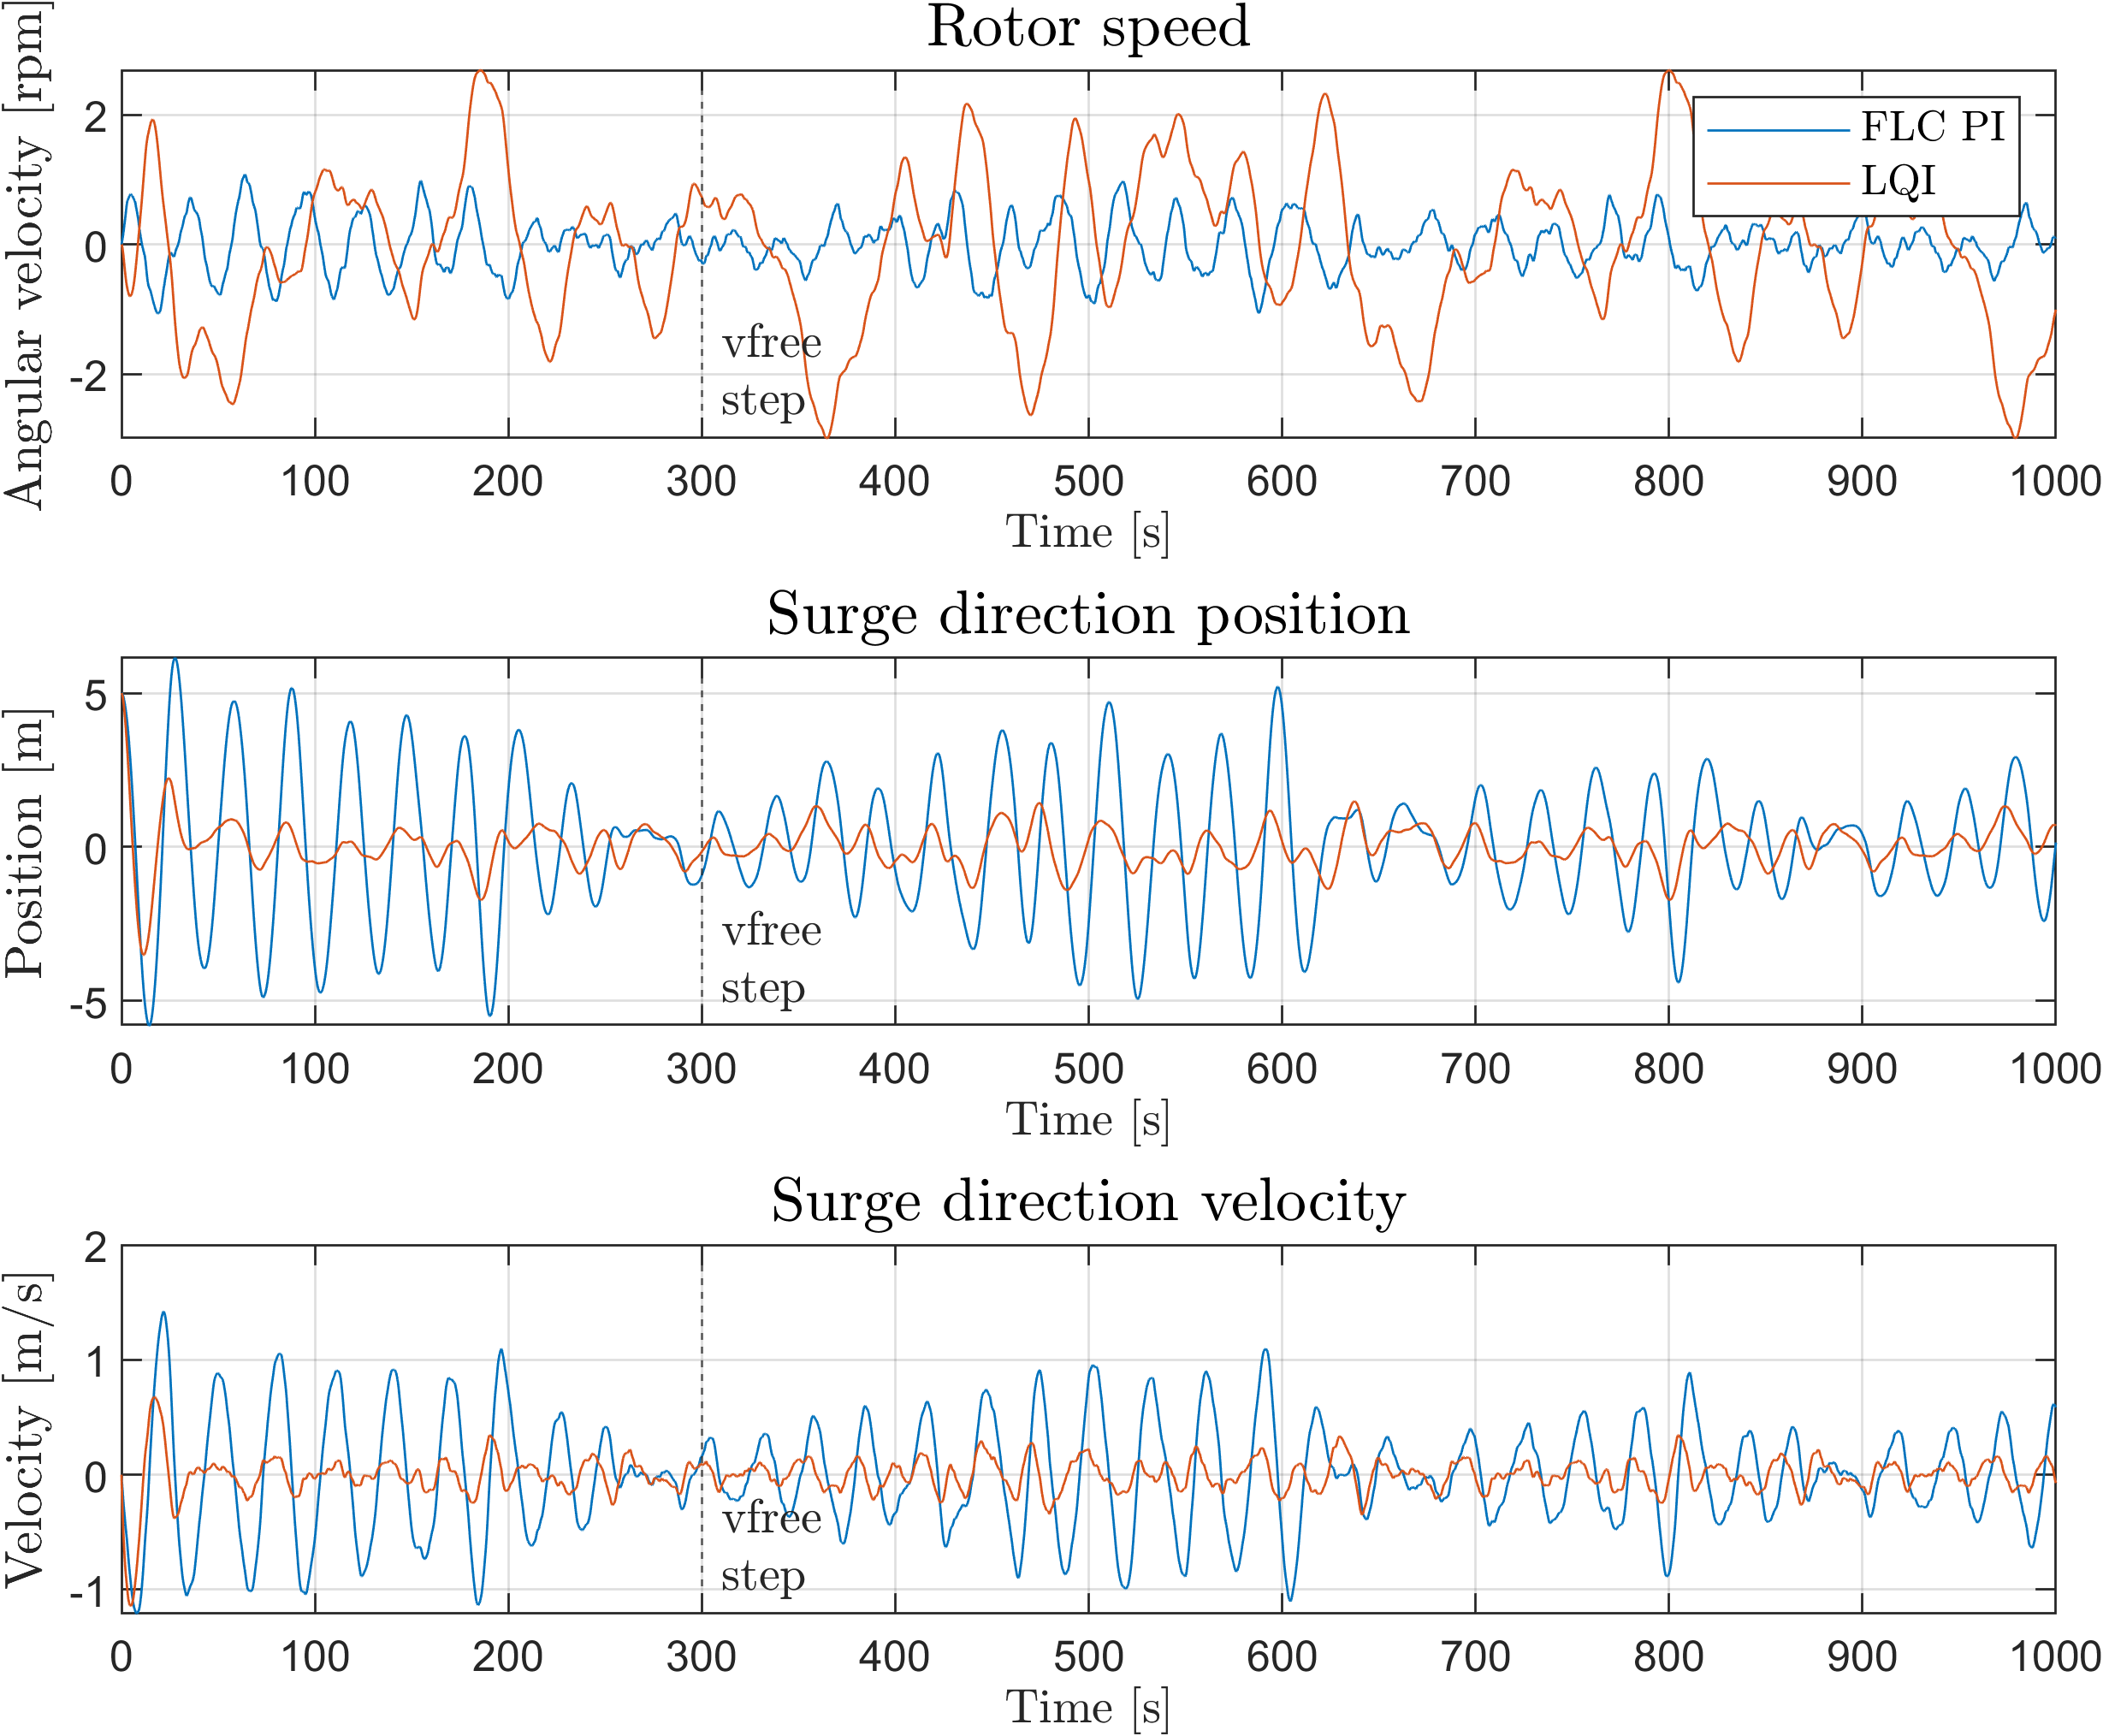
\includegraphics[width=0.7\linewidth]{Graphics/TestResults/linearModPerf/sim_02_W_py_vy_comp.png}
%	\caption{Simulink simulation results. The 10 m deviation initialization of the tower top position is visible from the \textit{fore-aft position} at 0 s.}
%	\label{fig:app_sim_02_W_py_vy_comp}
%\end{figure}
%
%\begin{figure}[ht]
%	\centering
%	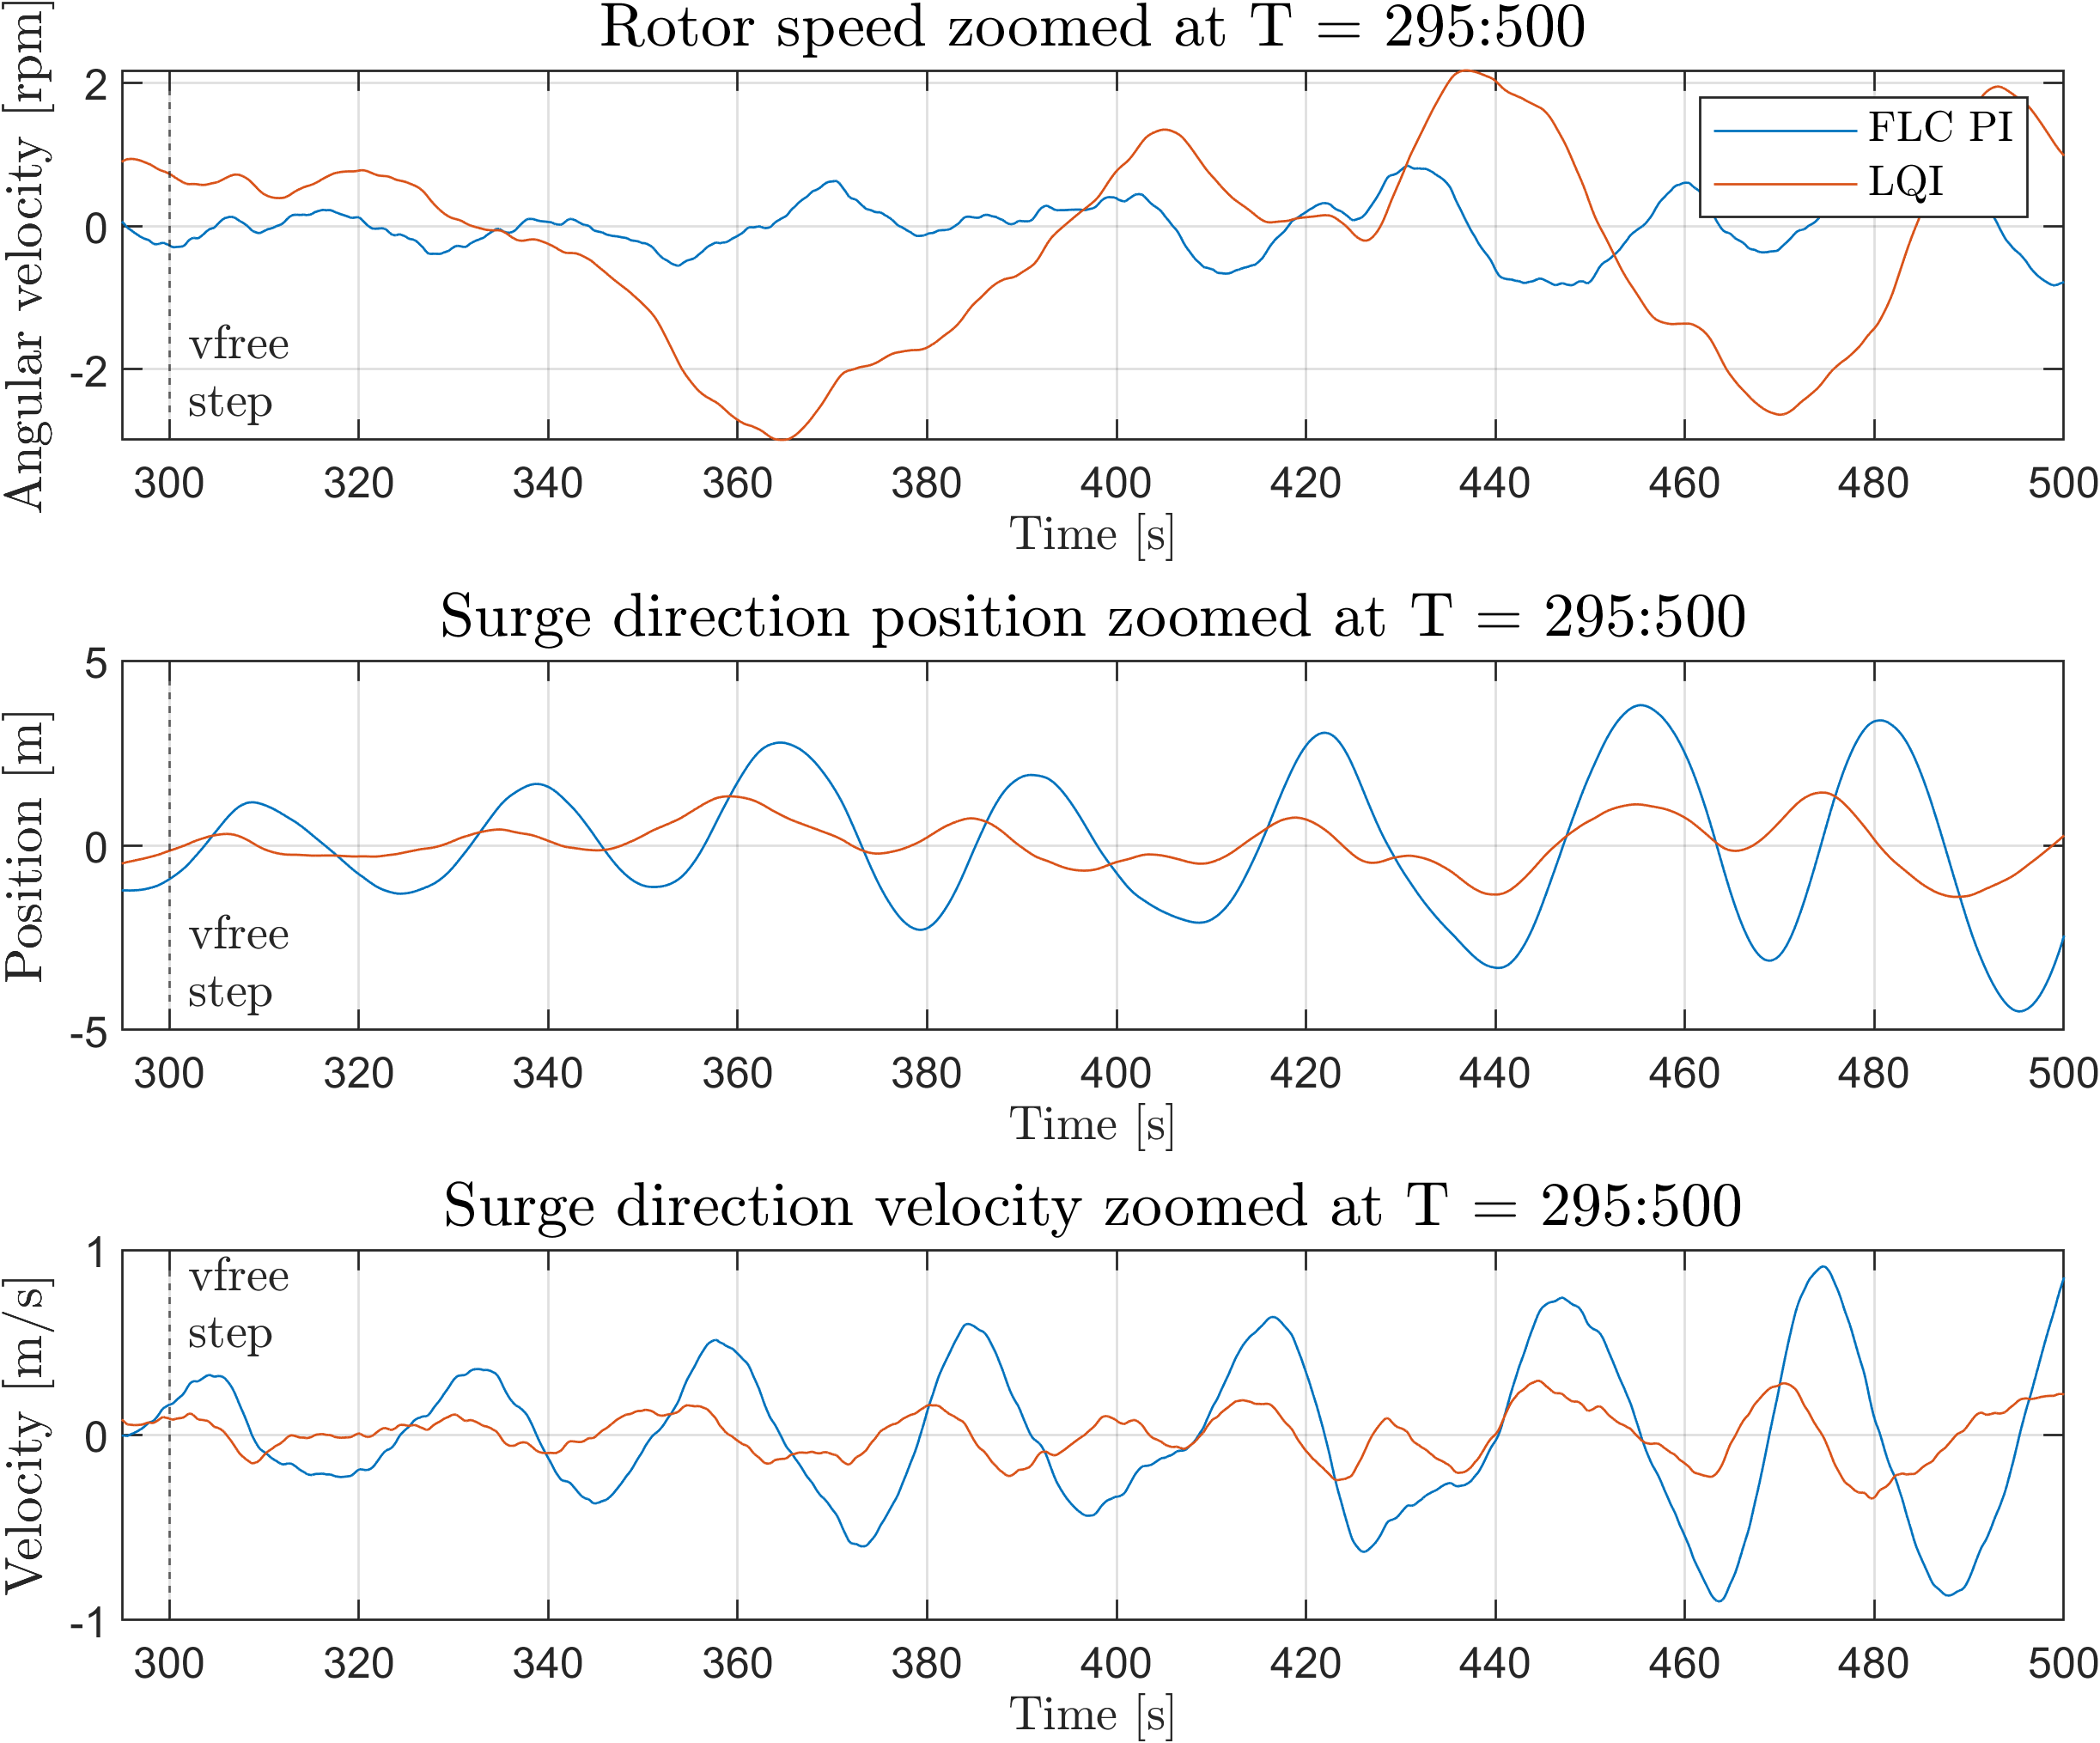
\includegraphics[width=0.7\linewidth]{Graphics/TestResults/linearModPerf/sim_03_W_py_vy_comp_zoom.png}
%	\caption{Simulink simulation results. Zoom at the disturbance step.}
%	\label{fig:app_sim_03_W_py_vy_comp_zoom}
%\end{figure}
%
%\begin{figure}[ht]
%	\centering
%	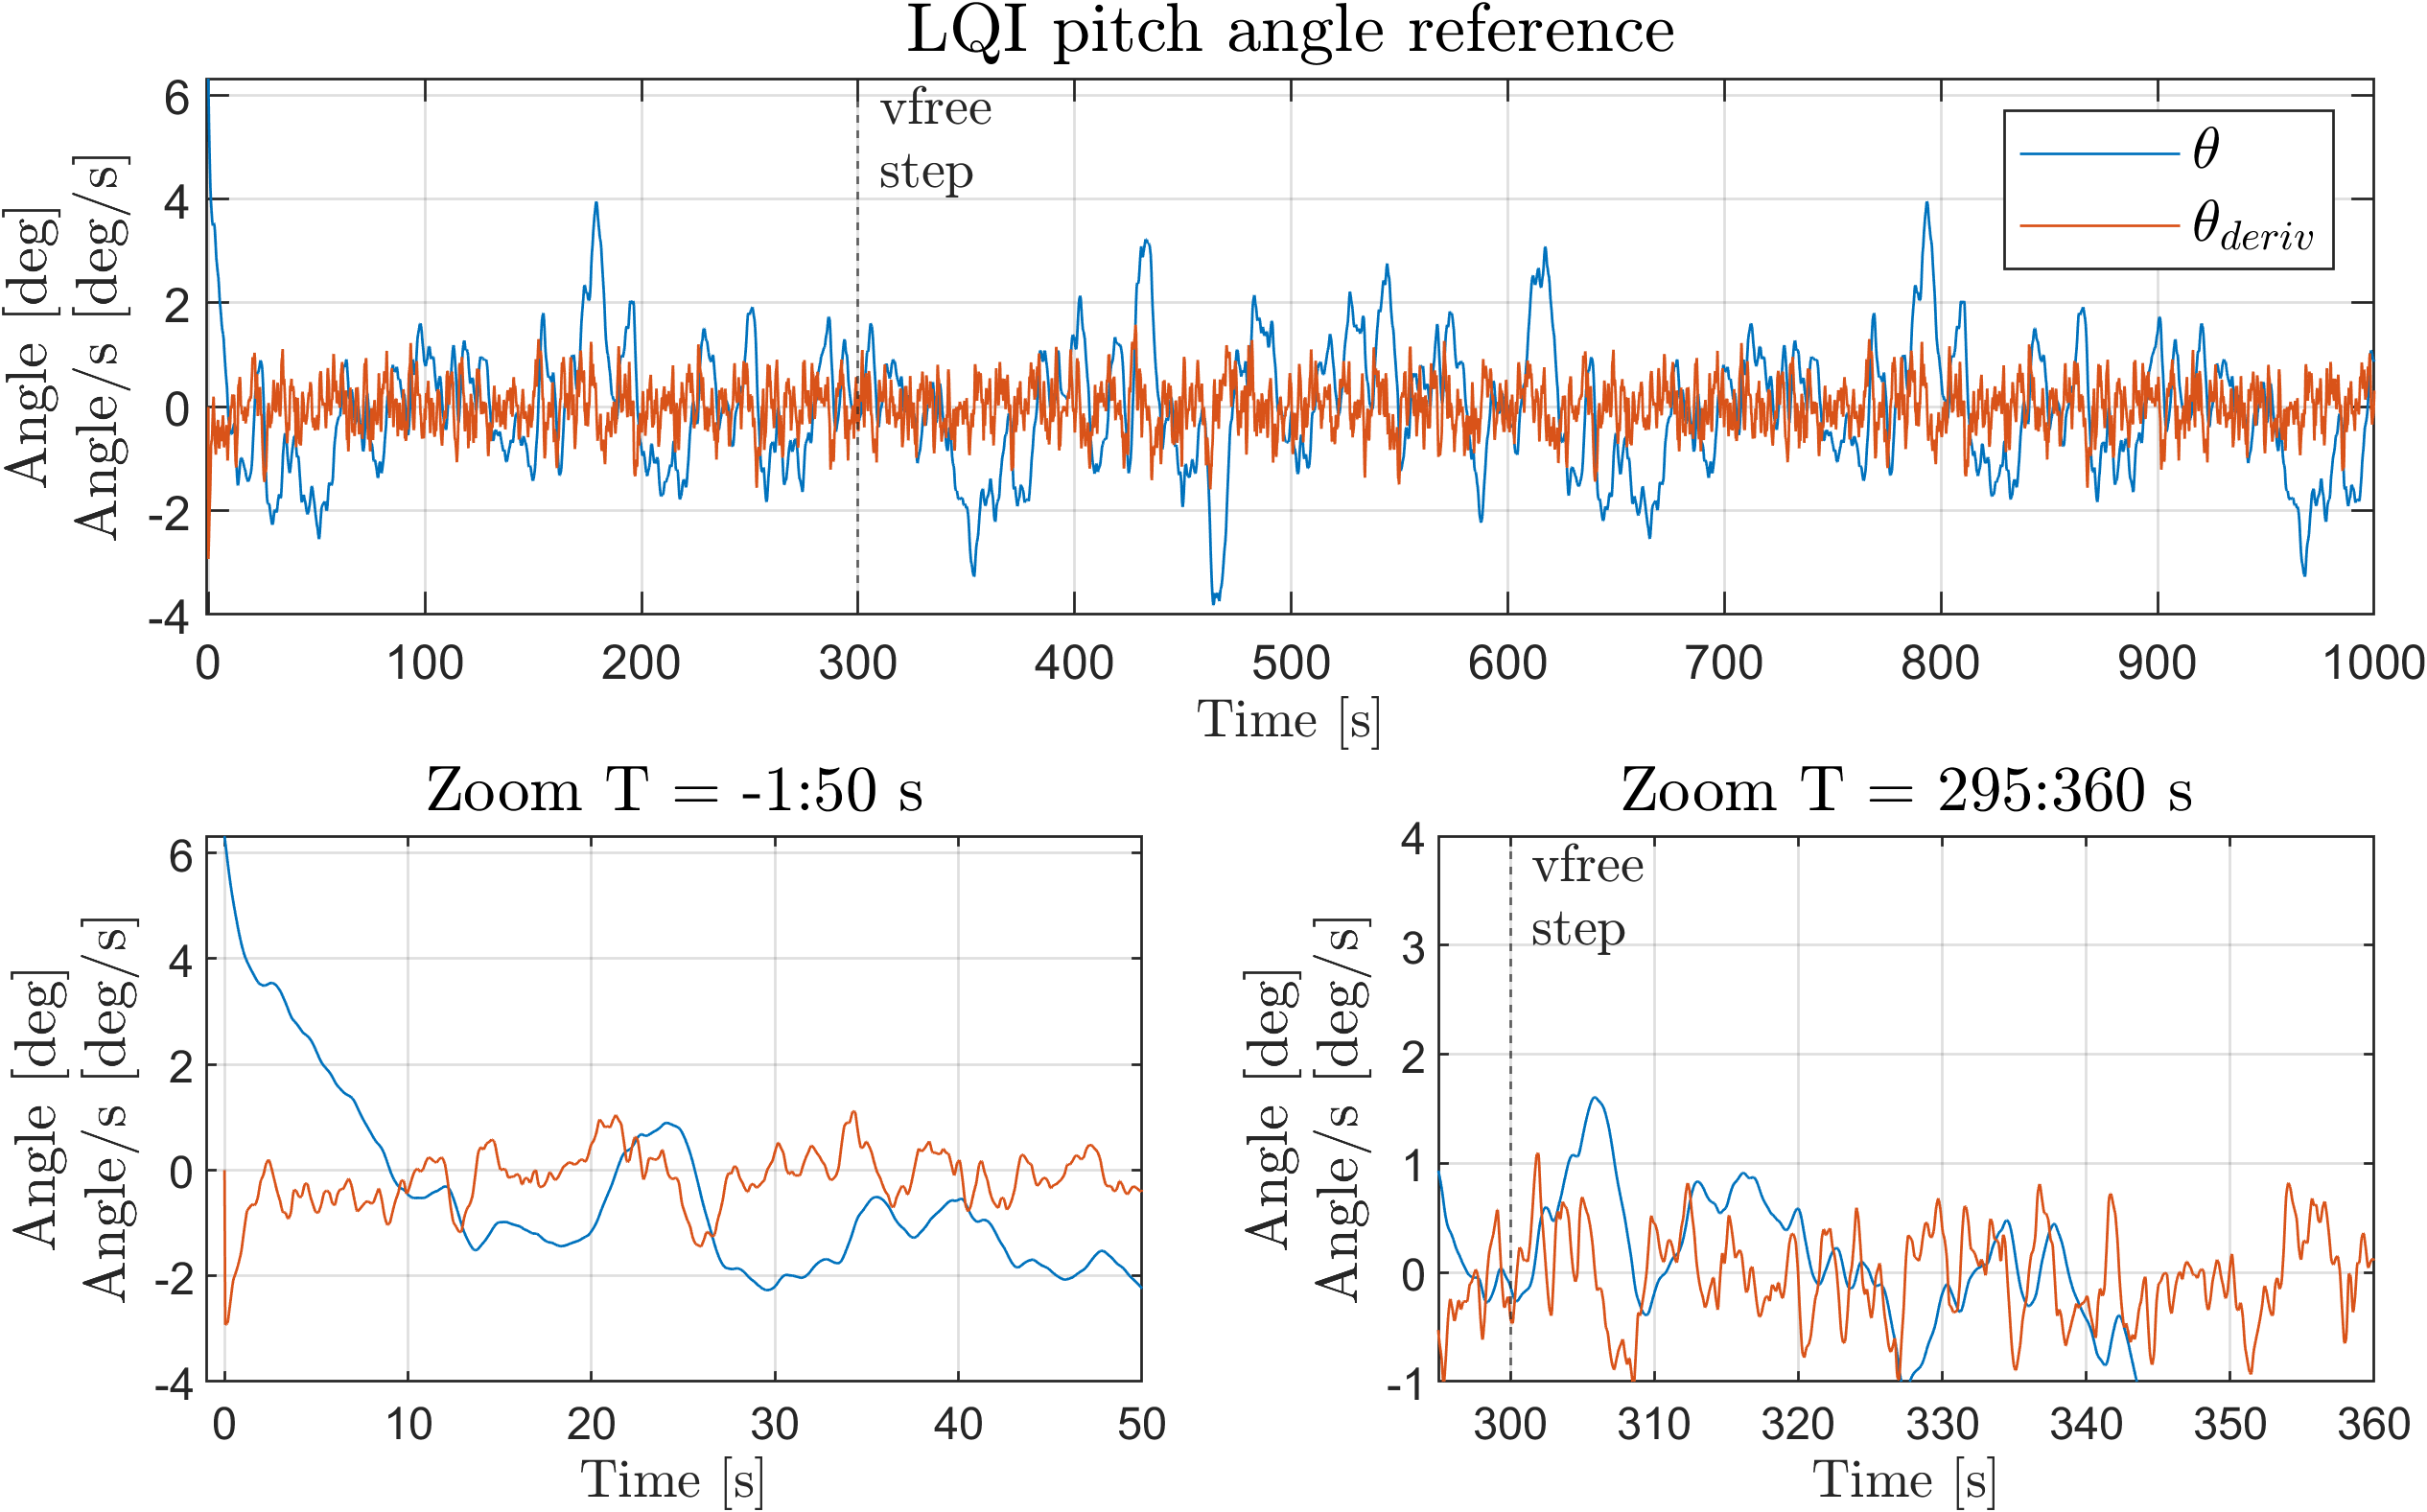
\includegraphics[width=0.7\linewidth]{Graphics/TestResults/linearModPerf/sim_01_pitch.png}
%	\caption{Simulink simulation results. Bottom left and right plots are zommed in at 0 to 50 s and 295 to 360 s.}
%	\label{fig:app_sim_01_pitch}
%\end{figure}


\subsection{Excluded component models} \label{sec:app_excl_comp_models}
This appendix contains component models which contain dynamics that from an understanding-the-theory POV are interesting but otherwise deemed unnecessary for the control objective. This is simply due to the frequency separation between the generally higher frequencies of these dynamics and the very slow eigenfrequency of a floating structure.

\subsubsection{Drivetrain (flexible)} \label{sec:mod_drt_flex}
As mentioned in \cref{sec:intro_wtcomponents} the drivetrain connects the rotor with the generator through a gearbox. The flexible drivetrain is modelled with a dampener and a spring between the rotor and the gearbox. The model is then reduced by translating the dampener and spring from the generator side to the rotor side of the gearbox. As such the model ends up consisting of two inertias coupled through a spring with stiffness $ K $ and a dampener with dampening $ B $. Due to the introduced spring and damper it is necessary to model both the rotor and and generator angle.
\begin{align} 
	J_{g} \ddot{\theta}_{gL} & = B (\dot{\theta}_r - \dot{\theta}_{gL}) + K(\theta_r - \theta_{gL}) - T_{g} \label{eq:comp_comp_drivetrain_flex_1} \\
	J_{r} \ddot{\theta}_r & = B (\dot{\theta}_{gL} - \dot{\theta}_r ) - K(\theta_r - \theta_{gL}) + T_{r} \label{eq:comp_comp_drivetrain_flex_2}
\end{align}
Recall the relationship between derivatives:
\begin{align}
	\dot{\Omega} & = \ddot{\theta}_r \\
	\dot{\omega}_{L} & = \ddot{\theta}_{gL} \\
	\dot{\theta}_g & = \omega \\
	\dot{\theta}_r & = \Omega
\end{align}
%and
%\begin{align}
%	\dot{\theta}_g & = \omega \\
%	\dot{\theta}_r & = \Omega
%\end{align}
and
\begin{align}
	\dot{\theta}_g 	&= \left(\dfrac{N_g}{N_r}\right) \dot{\theta}_{gL} \label{eq:comp_comp_drivetrain_flex_mod_3} \\
	J_{gL} 			&= J_{g} \left(\dfrac{N_r}{N_g}\right)^2 \label{eq:comp_comp_inertiamap_flex}
\end{align}
Which leaves the flexible drivetrain model as:
%\begin{align} 
%	\dot{\omega}_{gL} & = \dfrac{-B \dot{\theta}_{gL} + K(\theta_r - \theta_{gL}) - T_{g}}{J_{g}} \label{eq:comp_comp_drivetrain_flex_mod_1} \\
%	\dot{\Omega} & = \dfrac{-B \dot{\theta}_{gL} -B - K(\theta_r - \theta_{gL}) + T_{r}}{J_{r}} \label{eq:comp_comp_drivetrain_flex_mod_2} \\
%\end{align}
\begin{align} 
	\dot{\omega} & = \dfrac{B \left(\Omega - \dfrac{N_r}{N_g}\omega\right) + K\left(\theta_r - \dfrac{N_r}{N_g} \theta_{g}\right) - T_{g}}{\left(\dfrac{N_r}{N_g}\right)^2 J_{g} \dfrac{N_r}{N_g} } \label{eq:comp_comp_drivetrain_flex_mod_1} \\
	\dot{\Omega} & = \dfrac{B \left(\dfrac{N_r}{N_g}\omega - \Omega \right) \omega + K\left(\dfrac{N_r}{N_g} \theta_{g} - \theta_r\right) + T_{r}}{J_{r}} \label{eq:comp_comp_drivetrain_flex_mod_2} \\
	\dot{\theta}_g & = \omega \\
	\dot{\theta}_r & = \Omega
\end{align}
The model is observed to be linear and thus no linearisation is necessary.

The component inputs are $ \{T_g, T_r\} $ and the outputs are $ \{\omega, \Omega\} $. 

\subsubsection{Pitch system dynamics} \label{sec:comp_pitch_dyn}
The pitch system dynamics can be approximated with a simple first order low-pass filter which in the frequency domain is:
\begin{equation}\label{eq:comp_pitch_freq_dyn}
	\theta(s) = \dfrac{1}{\tau_{pit} s + 1} (\theta_{ref}(s) + \theta_{fatd}(s))
\end{equation}
where $ \tau_{pit} $ is a time-constant which suits the response of the pitching system at the operating point. In VTS the pitch system dynamics are modelled from a table which takes in the flap-wise bending moment of the blade and a pitch angle and outputs a pitch angle rate of change. As such wtLin uses the operating point and a user defined flap-wise bending moment to calculate $ \tau_{pit} $.

In the time domain the model becomes:
\begin{equation}\label{eq:comp_pitch_time}
	\dot{\theta} =\dfrac{(\theta_{ref}(s) + \theta_{fatd}(s)) - \theta}{\tau_{pit}}
\end{equation}

% The calculation of the time-domain version:
%\begin{align}\label{eq:comp_pitch}
%	\theta(s) & = \dfrac{1}{\tau_{pit} s + 1} (\theta_{ref}(s) + \theta_{fatd}(s)) \\
%	(\tau_{pit} s + 1) \theta(s) & = (\theta_{ref}(s) + \theta_{fatd}(s)) \\
%	\tau_{pit}\theta s + \theta(s)  & = (\theta_{ref}(s) + \theta_{fatd}(s)) \\
%	\tau_{pit}\dot{\theta} + \theta  & = (\theta_{ref}(s) + \theta_{fatd}(s)) \\
%	\dot{\theta} & =\dfrac{(\theta_{ref}(s) + \theta_{fatd}(s)) - \theta}{\tau_{pit}}
%\end{align}

The component inputs are $ \{\theta_{ref}, \theta_{fatd}  \} $ and the output is $ \{\theta \} $


\subsubsection{Generator} \label{sec:comp_generator_eff}
The generator is mechanically connected to the drivetrain and is electrically connected to the converter. It is used to control the rotor speed during PLC by means of the generator torque.

A more detailed generator model could include efficiencies. In Vestas' turbine simulator (VTS) the generator efficiencies are defined in tables and are dependent on grid output power $ P $ and generator speed $ \omega $. The output is three respective output efficiencies: 
\begin{enumerate}
	\item Mechanic efficiency: $ \eta_m(P,\omega) $
	\item Electric efficiency: $ \eta_e(P,\omega) $
	\item Auxiliary efficiency: $ \eta_a(P,\omega) $
\end{enumerate}
Where 
\begin{equation}\label{eq:comp_gen_effi_eff}
	\eta(P,\omega) = \eta_m(P,\omega) + \eta_e(P,\omega) + \eta_a(P,\omega)
\end{equation}
From the total efficiency the output grid power is:
\begin{equation}\label{eq:comp_gen_elec_pow_eff}
	P_{gen} \eta(P,\omega) = P
\end{equation}
where $ P_{gen} $ is the electrical power output of the generator.

This leaves the power loss from generator to grid to be defined as:
\begin{equation} \label{eq:comp_gen_pow_loss_eff}
	P_{loss}(P, \omega) = P_{gen} - P = \dfrac{P}{\eta(P, \omega)} - P
\end{equation}
The power of a rotating machine can be defined as the product of torque and rotational velocity:
\begin{equation}\label{eq:comp_power_in_rot_eff}
	P_{gen} = T_g \omega
\end{equation}
As such for the system at hand the torque can be defined by rearranging \cref{eq:comp_power_in_rot_eff} and substituting in $ P_{gen} $ from \cref{eq:comp_gen_pow_loss_eff}. This leaves the non-linear generator model to be:
\begin{equation}\label{eq:comp_gen_torque_eff}
	T_g(P, \omega) = \dfrac{P_{loss}(P, \omega) + P}{\omega}
\end{equation}
\cref{eq:comp_power_in_rot_eff} is the non-linear model of the generator. It contains $ P_{loss}(P,\omega) $ which from \cref{eq:comp_gen_pow_loss_eff} is dependent on $ \eta(P, \omega) $. The $ \eta $ function is extracted from VTS and linearized.

The linear model of the generator is obtained through a taylor expansion. The notation is relaxed a bit such that $ P_{loss}( P, \omega) $ is simply expressed as $ P_{loss} $.
\begin{equation}\label{eq:comp_taylor_eff}
	T_g( P, \omega) \approx T_g(P_o, \omega_o) + 
	\left. \dfrac{\partial T_g( P, \omega)}{\partial P} \right |_{P_o,\omega_o} ( P-P_o) + 
	\left. \dfrac{\partial T_g( P, \omega)}{\partial \omega} \right |_{P_o,\omega_o} (\omega - \omega_o)
\end{equation}
Below the the generator torque sensitivity to the grid power change term from \cref{eq:comp_taylor_eff} is derived. From \cref{eq:comp_gen_1_1_eff} to \cref{eq:comp_gen_1_2_eff} the \textit{sum rule} is used to split the derivative into two added derivatives. From \cref{eq:comp_gen_1_2_eff} to \cref{eq:comp_gen_1_3_eff} the first fractions in the denominators of the partial derivatives of the two terms are treated as a product of two functions thus the \textit{product rule} is used. The assumption is that the grid power is completely disconnected from the generator through the converter. Thus from \cref{eq:comp_gen_1_3_eff} to \cref{eq:comp_gen_1_4_eff} $ \, \frac{\partial \, \omega^{-1}}{\partial P} = 0 $.
\begin{align} 
	\dfrac{\partial T_g( P, \omega)}{\partial P} &= \dfrac{\partial \left (\dfrac{P_{loss} +  P}{\omega}\right )}{\partial P} \label{eq:comp_gen_1_1_eff} \\
	& = \dfrac{\partial \left (\dfrac{P_{loss}}{\omega} \right )}{\partial P} + \dfrac{\partial \left ( \dfrac{ P}{\omega} \right )}{\partial P} \label{eq:comp_gen_1_2_eff} \\
	& = \dfrac{1}{\omega} \cdot \dfrac{\partial P_{loss}}{\partial P} + \dfrac{\partial \left ( \dfrac{1}{\omega} \right )}{\partial P} P_{loss} + \dfrac{1}{\omega} \cdot \dfrac{\partial P}{\partial P} + \dfrac{\partial \left (\dfrac{1}{\omega} \right )}{\partial P}  P \label{eq:comp_gen_1_3_eff} \\
	& = \dfrac{1}{\omega} \cdot \dfrac{\partial P_{loss}}{\partial P} + \dfrac{1}{\omega} \label{eq:comp_gen_1_4_eff}
\end{align}


The generator torque sensitivity to rotational velocity change from \cref{eq:comp_taylor_eff} is then derived:
\begin{align}
	\dfrac{\partial T_g(P, \omega)}{\partial \omega} & = \dfrac{\partial \left (\dfrac{P_{loss} +  P}{\omega}\right )}{\partial \omega} \\
	& = \dfrac{\partial \left (\dfrac{P_{loss}}{\omega} \right )}{\partial \omega} + \dfrac{\partial \left (\dfrac{P}{\omega} \right )}{\partial \omega} \\
	& = \dfrac{1}{\omega} \cdot \dfrac{\partial P_{loss}}{\partial \omega} + \dfrac{\partial \left (\dfrac{1}{\omega} \right)}{\partial \omega} P_{loss} + \dfrac{1}{\omega} \dfrac{\partial P}{\partial \omega} + \dfrac{\partial \left (\dfrac{1}{\omega} \right )}{\partial \omega} P \\
	& = \dfrac{1}{\omega} \cdot  \dfrac{\partial P_{loss}}{\partial \omega} - \dfrac{1}{\omega^2}(P + P_{loss}) + \dfrac{1}{\omega} \dfrac{\partial P}{\partial \omega} \\
	& = -\dfrac{1}{\omega^2}(P + P_{loss}) + \dfrac{1}{\omega} \cdot \dfrac{\partial P_{loss}}{\partial \omega}
\end{align}
The above derived generator model is referred to the low-speed generator side by replacing $ \omega $ with $ \omega_L $ where $ \omega_L = \left (\frac{N_r}{N_g} \right ) \omega $. This yields the final linear generator model evaluated at the operating point $ (P_o, \omega_o) $. Furthermore $P_{loss}$ is still just a function of $ \omega_L $ and $ P $:
\begin{equation}
	\begin{split}
		T_g(P, \omega_L) 	& \approx \left. \left ( \dfrac{1}{\omega_L} \cdot \dfrac{\partial P_{loss}(P, \omega_L)}{\partial P} + \dfrac{1}{\omega_L} \right ) \right |_{P_o,\omega_{L_o}} (P - P_0) \\ 
		& + \left ( -\dfrac{1}{\omega_L^2}(P + P_{loss}(P, \omega_L)) + \left. \dfrac{1}{\omega_L} \cdot \dfrac{\partial P_{loss}(P, \omega_L)}{\partial \omega_L} \right ) \right |_{P_o,\omega_{L_o}} (\omega_L - \omega_{L_o})
	\end{split}
\end{equation}
The calculation of the power loss and derivation of the power loss sensitivity to grid power are left out here, but are calculated in wtLin at an operating point. In the wtLin tool these sensitivities are calculated based on the extracted tables of efficiency $ \eta $.

Presently the generator model in wtLin is implemented assuming a stiff drivetrain such that $ \Omega = \omega_L $.

The component model input is $ \{P, \Omega\} $ and the output is $ \{T_g\} $
